Ein wesentlicher Aspekt der K.I.\ ist es die aktuelle Spielfeldsituation der unterschiedlichen Spieler zu bewerten.
Dadurch kann die K.I.\ Spielz\"uge besser einstufen und gegebenenfalls das Spiel mit Spezialsteinen beeinflussen.
Ein naiver Ansatz w\"are der Vergleich der Anzahl an Spielsteinen jedes Spielers.
Dieses Vorgehen reicht jedoch nicht f\"ur eine ad\"aquate Bewertung der Spielsituation aus.
In Abbildung~\ref{fig:naivespielfeld01} w\"urde die naive Vorgehensweise den roten Spieler besser einstufen, jedoch hat er hier keinerlei m\"ogliche Spielz\"uge.
Der rote Spieler kann trotz dieser \"Uberlegenheit nicht mehr gewinnen, da der blaue Spieler im n\"achsten Spielzug \"uber alle roten Steine hinwegziehen kann.
Genau aus diesem Grund reicht eine naive Spielfeldbewertung nicht f\"ur ein aussagekr\"afigtes Resultat aus.

\vspace{1em}
\begin{minipage}{\linewidth}
    \centering
    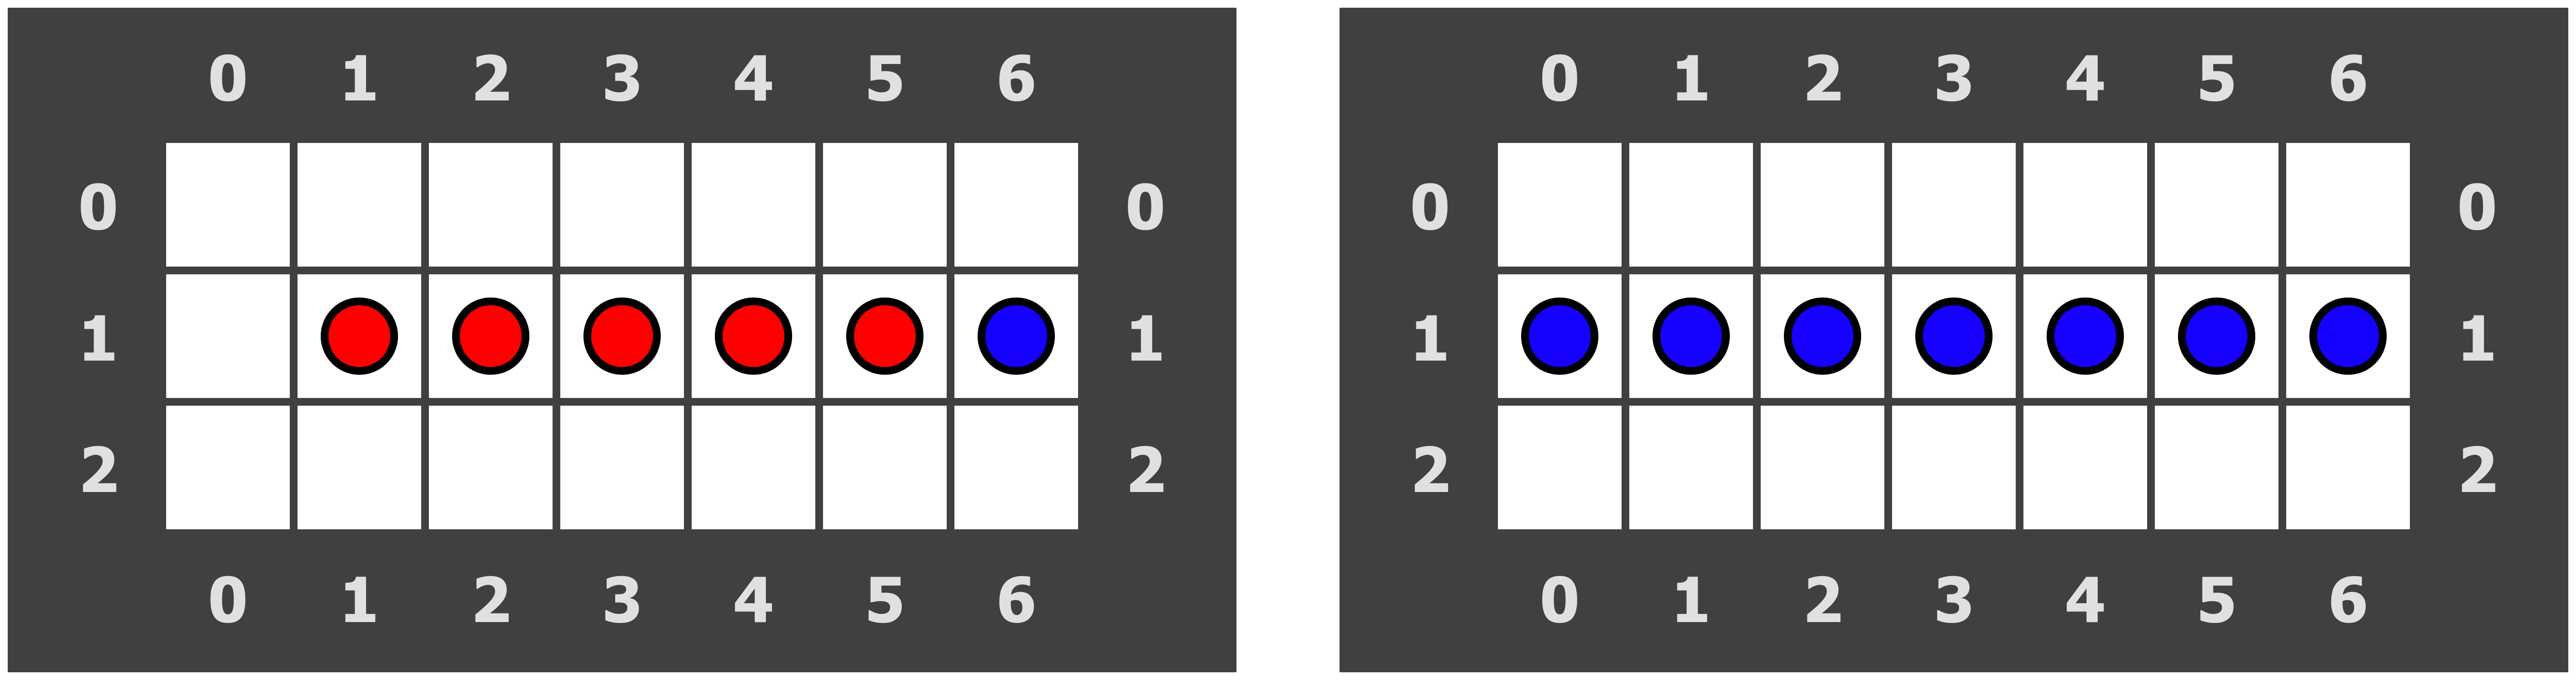
\includegraphics[width=0.6\linewidth]{pics/naive-game-situation}
    \captionof{figure}{Problematik der naiven Bewertung}
    \label{fig:naivespielfeld01}
\end{minipage}

\subsection{Bestandteile der Heuristik}\label{subsec:bestandteile-der-heuristik}
Wie bereits in der Einleitung dieses Abschnitts begr\"undet, gen\"ugt das reine Abz\"ahlen der Spielsteine nicht aus.
Deshalb setzt dieser Client auf drei unterschiedliche Heuristikbestandteile, um die aktuelle Spielsituation zu bewerten.
Unter diesen drei Ans\"atzen werden die \emph{Mobilit\"at} der Spieler, das \emph{Verh\"altnis der Spielsteine} sowie die aktuelle \emph{Bewertung der Karte} miteinbezogen.
Diese einzelnen Bestandteile sind w\"ahrend des Spiels jedoch nicht immer gleichbedeutend.
Zu Beginn muss darauf geachtet werden, dass man sehr flexibel bleibt und Positionen erobert die sp\"ater nur schwer einnehmbar sind.
Hierzu z\"ahlen vor allem Ecken und Kanten.
Erobert man nun ein solches Feld, wird der Gegner in seiner Zugwahl eingegrenzt, da er keine Z\"uge w\"ahlen will, die bereits einen Zug sp\"ater wieder \"uberzogen werden.
Eine solche Situation schr\"ankt die Mobilit\"at des Gegners drastisch ein und auch die Bewertung des Spielers aufgrund seines Kartenwertes leidet darunter.
Je weiter man sich jedoch dem Spielende n\"ahert, desto unwichtiger wird dieses Bewertungskriterium.
Dies liegt daran, dass man das Spiel nicht aufgrund hoher Mobilit\"at gewinnt, sondern anhand der Anzahl seiner Spielsteine.
Aus diesem Grund wird das Verh\"altnis der Spielsteine zum Ende hin immer wichtiger.
Ma"sgeblich ist nun den prozentualen Spielverlauf abzusch\"atzen, um damit die einzelnen Heuristikbestandteile akkurat gewichten zu k\"onnen.

\subsubsection{Gewichtung des Spielfeldes}\label{subsubsec:gewichtung-des-spielfeldes}
Es gibt gewisse Positionen die f\"ur einen Spieler wertvoller sind als andere.
Zu diesen Positionen z\"ahlen unter anderem Kanten und Ecken, da es wesentlich schwieriger, bis garnicht m\"oglich ist, diese einzunehmen.
Eine Ausnahme stellt hier das Einnehmen mithilfe von \"Uberschreib-, bzw.\ Spezialsteine dar.
Insbesondere sind Felder die zwei Felder oder mehr von einem Bonusfeld in direkter Richtung entfernt sind h\"oher gewichtet, da sie die M\"oglichkeit geben einen solchen Bonusstein einzunehmen falls ein Gegner auf ein direktes Nachbarfeld des Spezialfeldes zieht.

\vspace{1em}
\begin{minipage}{\linewidth}
    \centering
    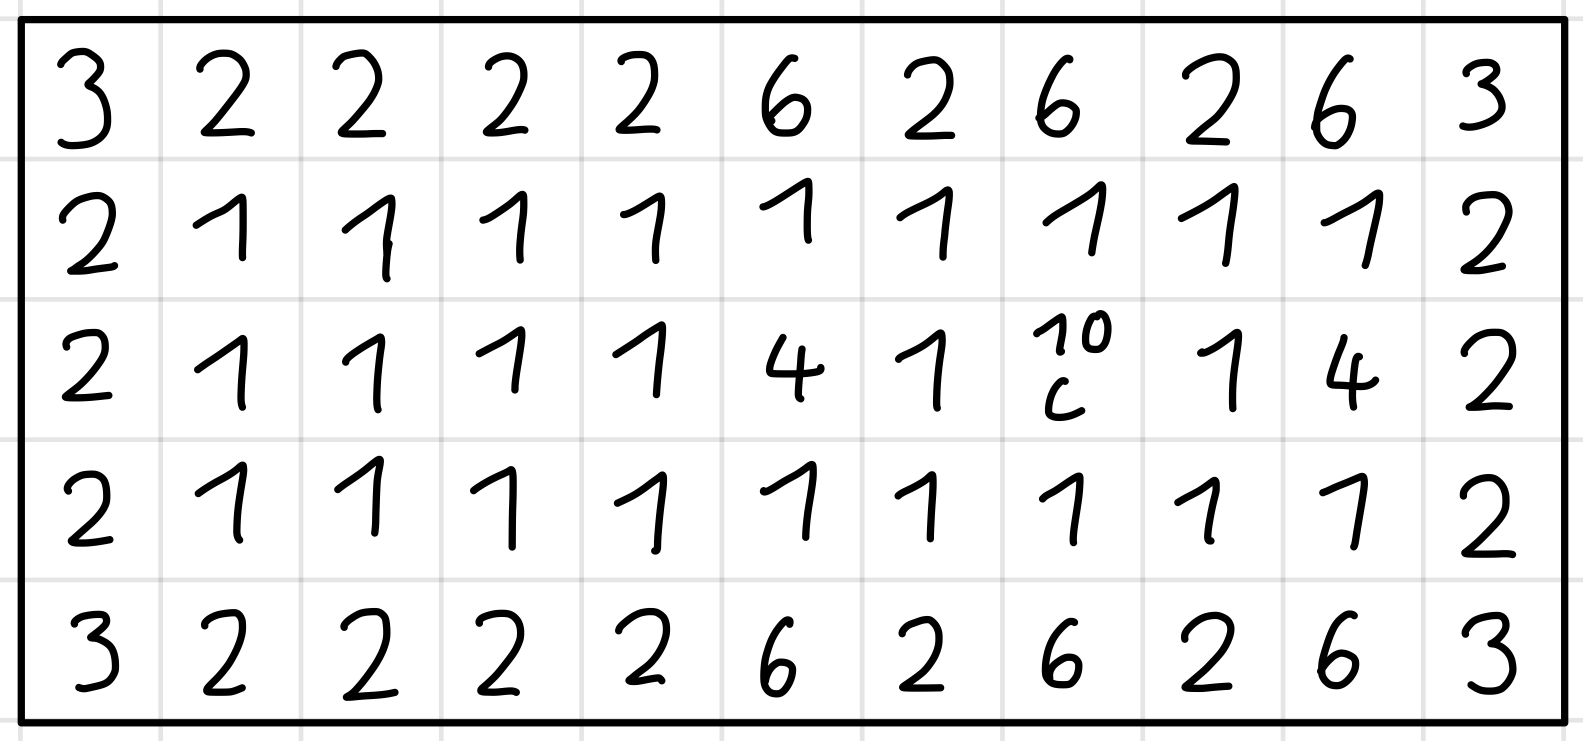
\includegraphics[width=0.5\linewidth]{pics/rating}
    \captionof{figure}[Bewertungsverfahren 01]{Spielfeldpositionen mit Gewichtungen}
    \label{fig:bewertungsverfahren01}
\end{minipage}

Der Score eines Spielers setzt sich dann aus der Summe der belegten Felder mit der entsprechenden Gewichtung zusammen.

Dieses Bewertungsverfahren bietet Vor- und Nachteile.
Positiv daran ist, dass bei Beginn des Spieles jedem Feld eine Gewichtung zugeteilt wird und diese nur noch durch erreichen von Spezialfeldern geringf\"ugig ge\"andert wird.
Negativ ist jedoch, dass dieses Bewertungsverfahren besonders bei gro"sen rechteckigen Spielfeldern mit wenig Spezialfeldern ann\"ahernd wie die naive Variante funktioniert.

\subsubsection{Mobilit\"at}\label{subsubsec:mobilitaet}
Ein weiterer Bestandteil der Analyse besteht darin, Spielsituationen anhand der Beweglichkeit der Spieler einzustufen.
Hierbei wird die Anzahl an Spielz\"ugen eines jeden Spielers bestimmt und miteinander verglichen.
Wie bereits in der Einleitung gezeigt kann ein Spieler seine positive Stellung nur halten, solange er weiterhin spielf\"ahig bleibt.
Aus diesem Grund wird in diesem Ansatz bestimmt wie beweglich ein Spieler gegen\"uber den Anderen ist.

Ein Vorteil dieser Bewertungsmethode besteht darin, dass ein Spieler mit wenig Steinen aber einer hohen Mobilit\"at bei diesem Verfahren nicht negativ bewertet wird.
Ein Problem daran ist jedoch, dass zum Ende des Spieles dieser Ansatz an Relevanz verliert, da zum Schluss nur die Anzahl an eigenen Steinen relevant ist.

\subsubsection{Spielfeldbelegung}\label{subsubsec:spielfeldbelegung}
Da es besonders gegen Ende des Spiels essenziell ist, viele Steine zu besitzen, muss man dies ebenfalls in die Bewertung miteinbeziehen.
Anstatt aber nur einfach die Anzahl der Spielsteine zu z\"ahlen, wird hier das prozentuale Verh\"altnis gegen\"uber allen existierenden Spielsteinen genommen.

Der Vorteil dieses Verfahrens ist hier, dass man vor allem im sp\"ateren Spielverlauf feststellen kann, wie der aktuelle Stand des Spiels ist und welche Spieler es anzugreifen gilt.
Der Nachteil hierbei ist aber, dass dieses Verfahren im anf\"anglichen und mittleren Spielverlauf nicht aussagekr\"aftig ist.
Dies liegt daran, dass man besonders zum Spielende durch eine zuvor sehr gute Mobilit\"at einen vermeintlich besseren Spieler sehr viele Steine wegnehmen kann.
Allerdings muss man diese Berechnung wie Anfangs erw\"ahnt mit einflie"sen lassen, da man zum Schluss einen Greedyansatz w\"ahlen muss.
Denn letztlich ist f\"ur das Gewinnen des Spieles nur die Anzahl an Spielsteinen von Bedeutung.

\subsection{Algorithmen der Zugauswahl}\label{subsec:algorithmen-der-zugauswahl}
F\"ur einen Computer ist es unm\"oglich den besten Spielzug zu finden, da hier jedes m\"ogliche Spielfeld \"uberpr\"uft werden m\"usste.
Bei einem Spiel wie Schach w\"aren dies circa $10^{120}$ unterschiedliche Spielbrettzust\"ande~\cite{chessBoards}.
Bei ReversiXT liegt die Zahl wesentlich h\"oher, da es zum einen viel gr\"o"sere Karten und zum anderen bis zu 8 Spieler gibt.
Damit ein Computer trotzdem einen guten Zug abliefern kann werden spezielle Algorithmen ben\"otigt.
Ein weit verbreiteter Algorithmus f\"ur Zwei-Personen-Nullsummenspiele\footnote{Duden: Spiel, bei dem die Summe der Einsätze, Verluste und Gewinne gleich null ist} lautet Minimax.

\subsubsection{Minimax Algorithmus}\label{subsubsec:minimax-algorithmus}
Zur Veranschaulichung von Minimax soll ein kurzes Gedankenexperiment (siehe Abbildung~\ref{fig:thought-experiment}) dienen.
Es gibt zwei Personen.
Die eine hat zwei Schubl\"aden A \& B mit je zwei Gegenst\"anden (Wert in Euro angegeben).
Die andere Person darf sich nun eine Schublade aussuchen, aus dem Sie ein Geschenk bekommt.
Nun muss der Besitzer dieser Gegenst\"ande ausw\"ahlen, welches er dem Gl\"ucklichen \"uberreichen m\"ochte.
Deshalb wird er den Gegenstand w\"ahlen, der f\"ur Ihn am wenigsten Verlust darstellt.
Aus diesem Grund ergibt es f\"ur den Spieler YOU keinen Sinn die Schublade B auszuw\"ahlen, da man hier den Gegenstand f\"ur 1~\euro{} bekommt, andernfalls den f\"ur 20~\euro{}.

\vspace{1em}
\begin{center}
    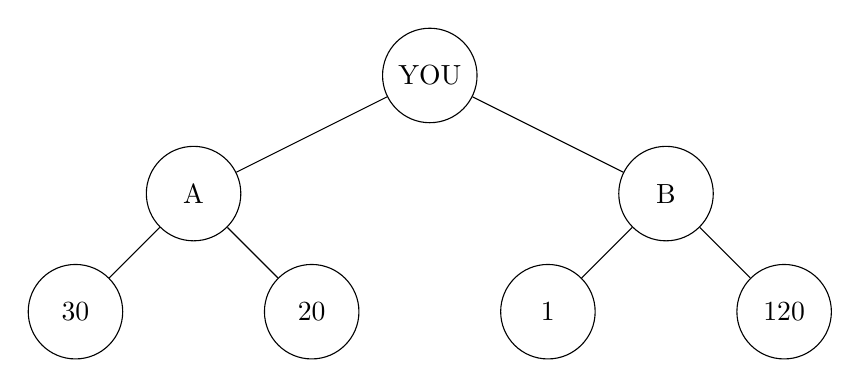
\begin{tikzpicture}[sibling distance=10em,
        every node/.style={circle, draw, minimum size=1.2cm},
        level/.style={sibling distance=6cm/#1}]

        \node (Root) {YOU}
        child {
            node {A}
            child { node {30} }
            child { node {20} }
        }
        child {
            node {B}
            child { node {1} }
            child { node {120} }
        };

    \end{tikzpicture}
    \captionof{figure}{Grafik zur Veranschaulichung des Gedankenexperimentes}
    \label{fig:thought-experiment}
\end{center}

Ein solches Verfahren kann nun genutzt werden um unterschiedliche Spielz\"uge zu vergleichen und den Bestm\"oglichen - unter Ber\"ucksichtung der sp\"ateren Z\"uge des Gegners - auszuw\"ahlen.
Jedoch beinhaltet dieser Algorithmus einen Nachteil - es werden auch Spielz\"uge betrachtet, die nicht infrage kommen, da ein Spieler diesen Zug niemals w\"ahlen wird.

\subsubsection{Alpha-Beta-Pruning}\label{subsubsec:alpha-beta-pruning}
Dieses Problem kann mithilfe des Alpha-Beta-Prunings drastisch reduziert werden.
Hierbei werden Hilfsvariablen (alpha und beta) durchgereicht.
Dieser Verbesserung muss Zugfolgen, die das Ergebnis unbeeinflusst lassen, nicht mehr kontrolliert.
Beim Gedankenexperiment muss somit nach dem Gegenstand im Wert von 1~\euro{} kein weiterer Knoten untersucht werden, da der Spieler YOU diesen Pfad (im Beispiel die Schublade B) nicht w\"ahlen wird.
Das liegt daran, dass f\"ur ihn die Schublade A wesentlich interessanter ist.
Selbstverst\"andlich nur unter Ber\"ucksichtigung, dass der Andere seinen Verlust minimieren m\"ochte.

\subsubsection{Vergleich der Algorithmen}\label{subsubsec:vergleich-der-algorithmen}
Um die Bedeutung dieser Variante zu verdeutlichen, folgt nun ein Vergleich beider Verfahren.
Dabei wird zuerst dieselbe Karte mit unterschiedlichen Suchbaumtiefen getestet.
Es treten in den Tiefen 3 bis 8 jeweils zwei Spieler gegeneinander an\footnote{Die Suchbaumtiefe 8 wurde auf einem Labor-PC der OTH Regensburg durchgef\"uhrt. N\"ahere Informationen siehe Kapitel~\ref{subsec:technische-daten}}.
Es wird je einmal der erste Spieler und einmal der zweite Spieler mit Alpha-Beta gestartet.

\vspace{1em}
\begin{minipage}{\linewidth}
    \centering
    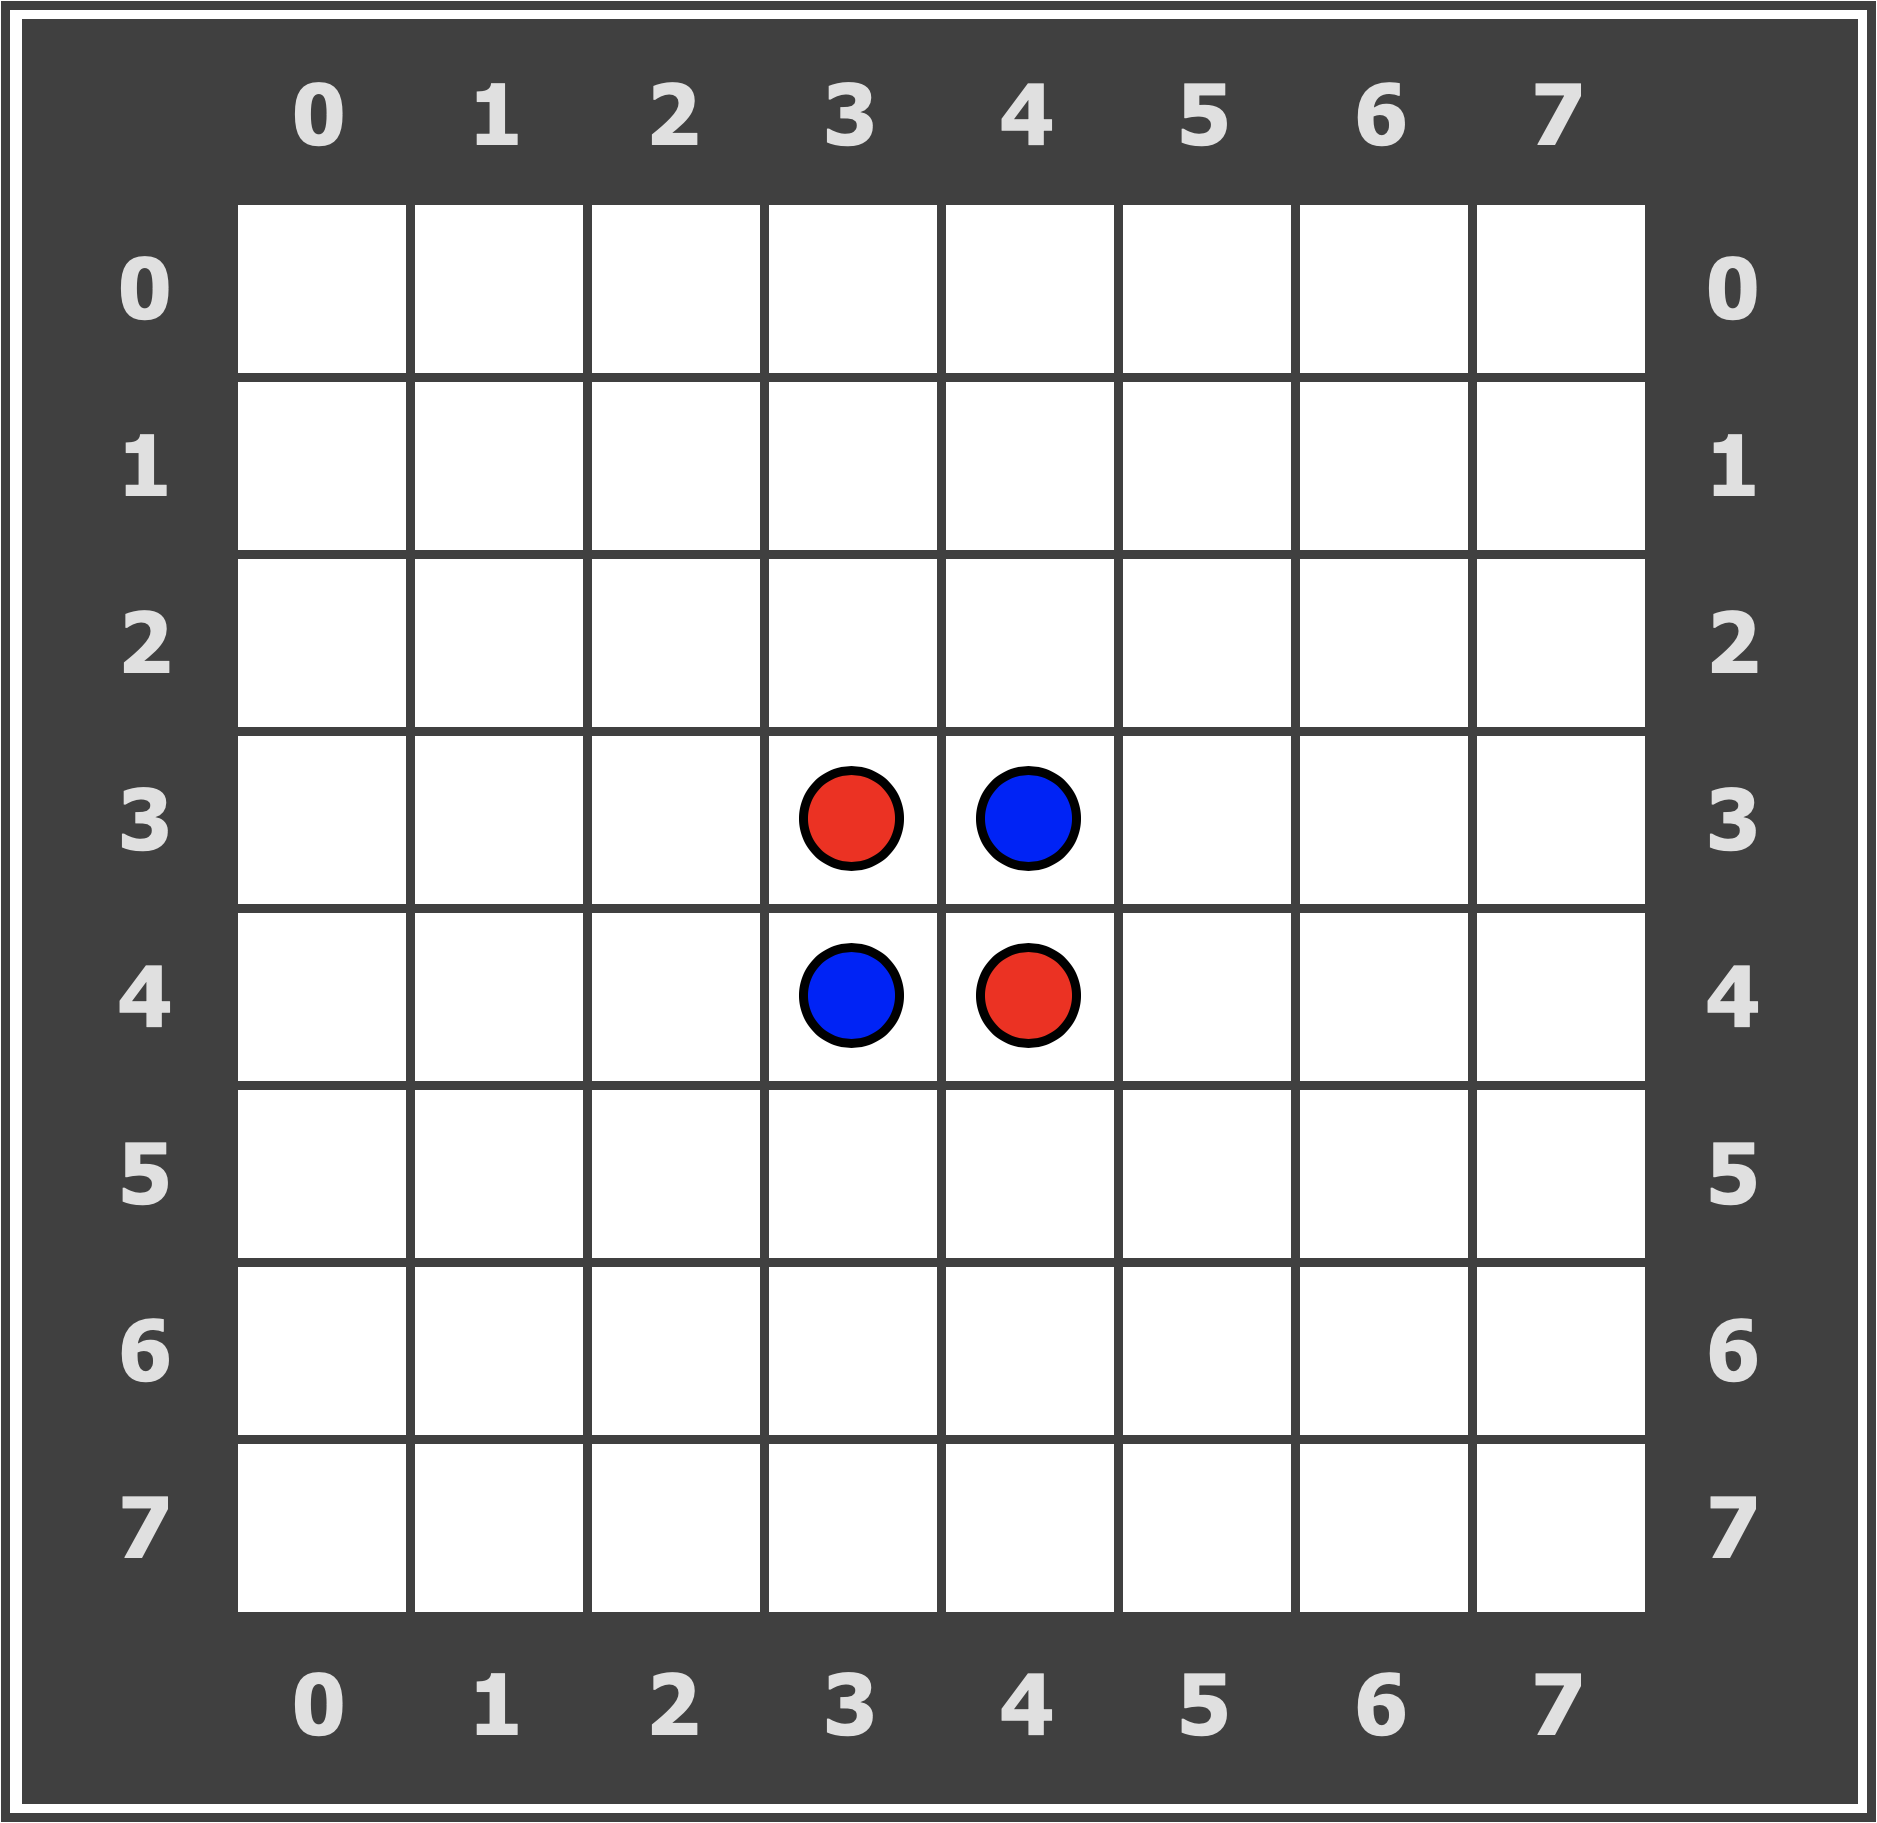
\includegraphics[width=0.3\linewidth]{pics/statistic-map}
    \captionof{figure}[Karte für Statisitk]{Verwendete Karte für den Vergleich von Minimax und Alpha-Beta}
    \label{fig:statistic-map}
\end{minipage}

Es wird aus folgenden Gr\"unden die Karte aus Abbildung~\ref{fig:statistic-map} zu Begin gew\"ahlt:
\begin{enumerate}
    \item Es gibt nur zwei Spieler, womit beide Verfahren gegeneinander antreten k\"onnen.
    \item Es gibt keine Spezialsteine, was das Spiel einfacher gestaltet und beim Vergleich der Algorithmen nicht von Bedeutung ist.
    \item Die verwendete Karte ist komplett symmetrisch, wodurch eine Fairness f\"ur beide Spieler garantiert wird.
    \item Es handelt sich um eine relativ kleine Karte, damit die Berechnungen zeitlich einigerma"sen eingegrenzt werden k\"onnen.
\end{enumerate}

\vspace{1em}
\begin{minipage}{\linewidth}
    \centering
    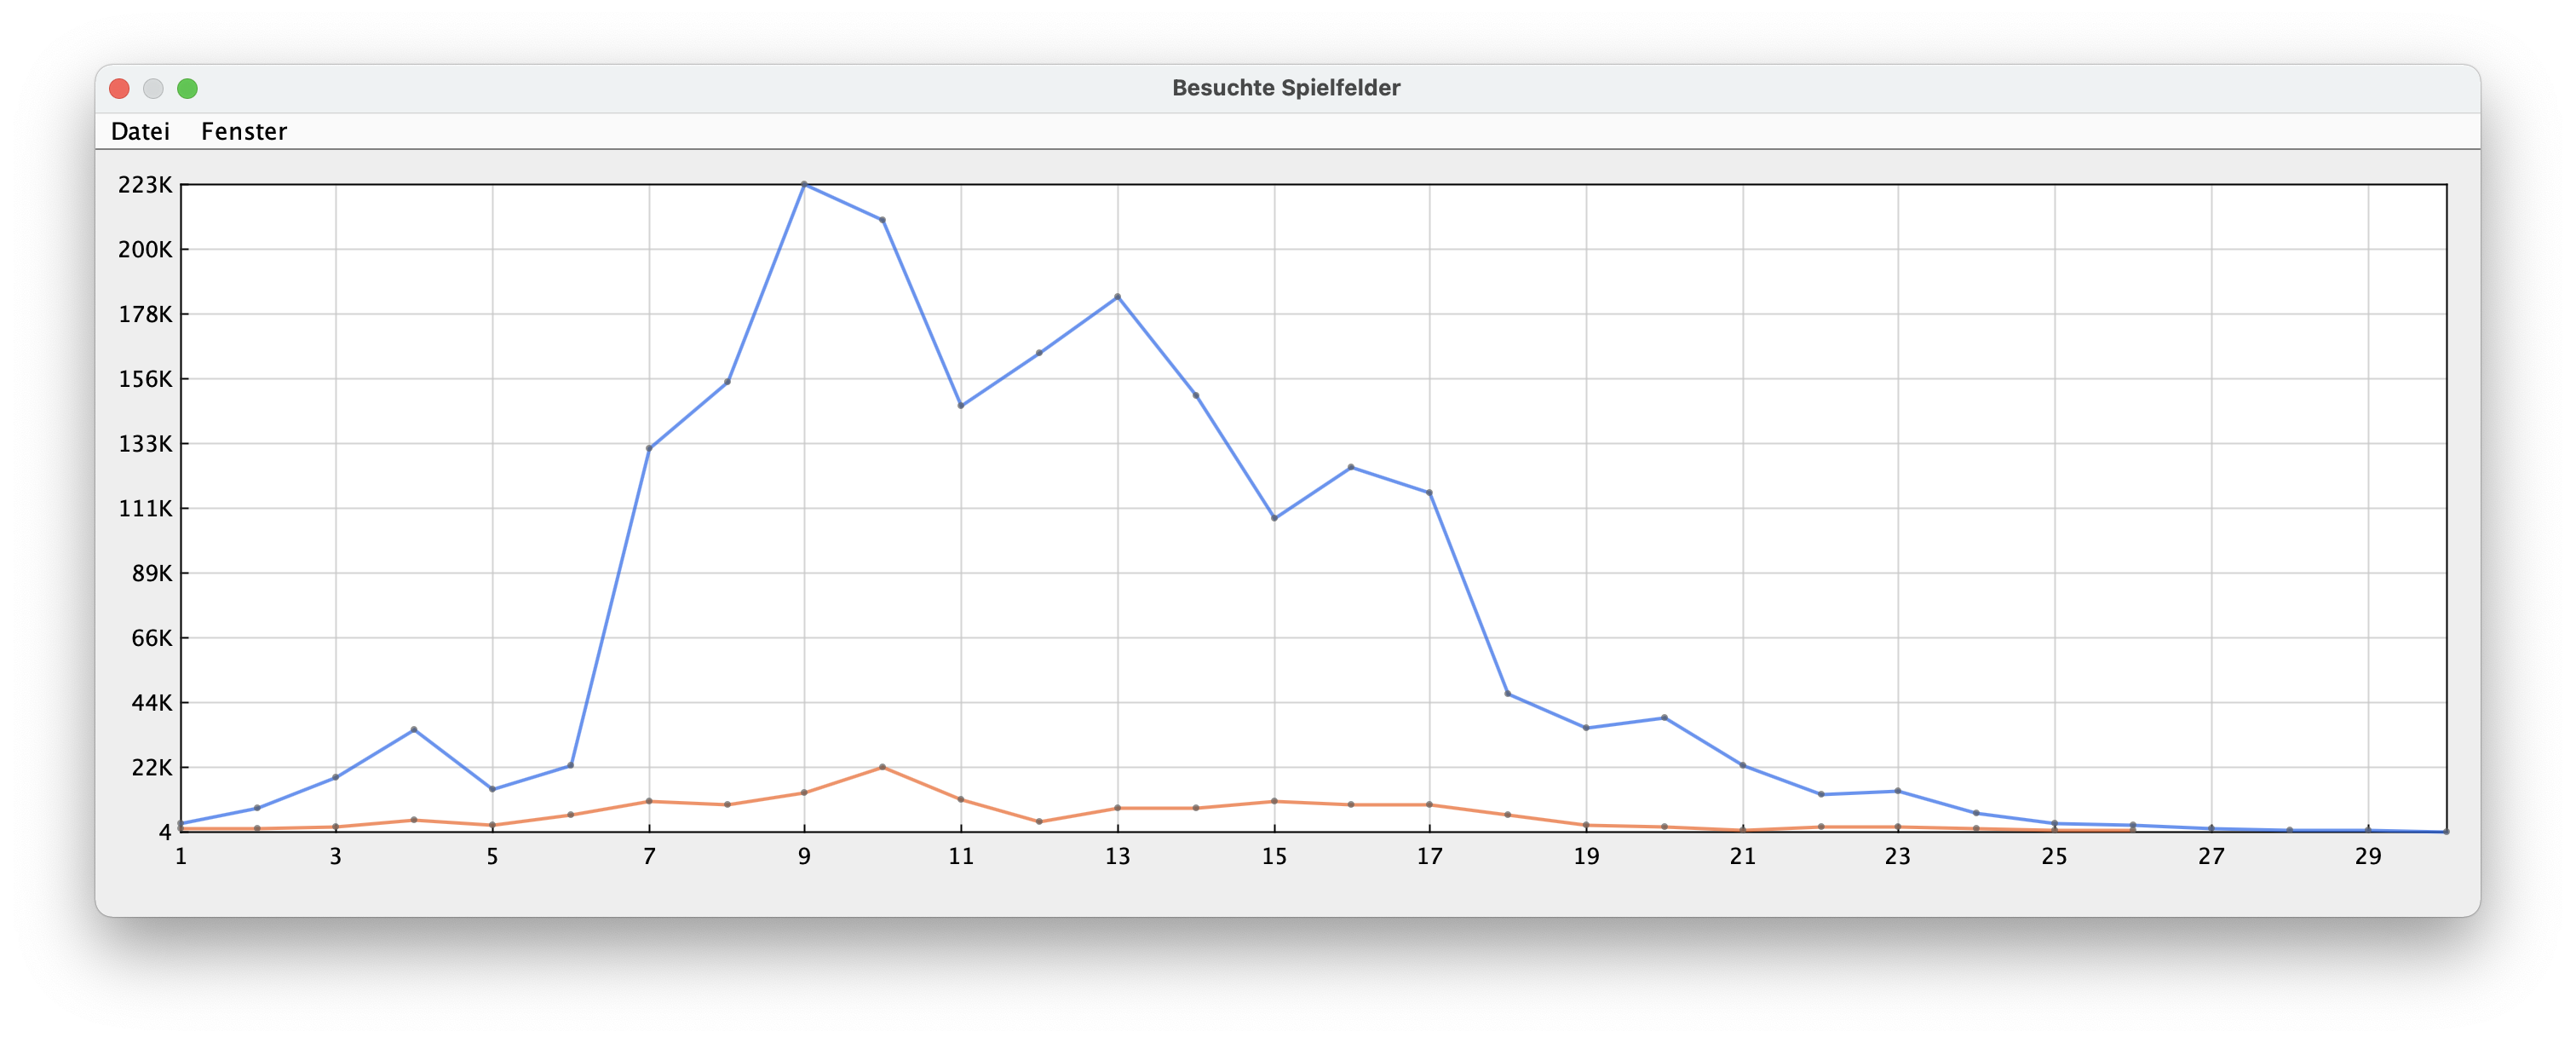
\includegraphics[width=0.9\linewidth]{statistic/ORIGINAL-D5-01/ST-01-D5-LD}
    \captionof{figure}[Statistik für Tiefe 5]{Diese Statistik wurde bei einem Spiel der Tiefe 5 aufgenommen.}
    \label{fig:statistic-screen}
\end{minipage}

In Abbildung~\ref{fig:statistic-screen} sind sowohl \"uberpr\"ufte Karten ohne Alpha-Beta (blaue Linie), als auch mit Alpha-Beta (orange Linie) zu sehen.
Hierbei ist klar ersichtlich, dass Alpha-Beta-Pruning einen enormen Leistungsvorteil liefert.
Der obige Screenshot stammt aus der selbstentwickelten Software GameAnalyzer.
Mehr dazu in Kapitel~\ref{sec:spielanalyse}.

Die Tabelle~\ref{tab:search-depth} liefert eine \"Ubersicht \"uber alle getesteten Suchbaumtiefen dieser Karte.

\vspace{1em}
\begin{table}[!h]
    \centering
    \begin{tabular}{|l|c|c|}
        \hline
        \textbf{Tiefe} & \textbf{Alpha-Beta} & \textbf{Minimax}\\
        \hline
        3 & 1.079,5 & 2.434,5\\
        \hline
        4 & 5.985,5 & 18.417,5\\
        \hline
        5 & 22.653 & 244.854,5\\
        \hline
        6 & 133.657,5 & 1.313.347\\
        \hline
        7 & 419.537 & 28.802.230\\
        \hline
        8 & 1.898.497 & 449.424.275\\
        \hline
    \end{tabular}
    \caption{Besuchte Karten mit den Suchalgorithmen (Ergebnisse wurden geglättet)}
    \label{tab:search-depth}
\end{table}

Auf den ersten Blick wirken diese Zahlen nun ziemlich bedeutungslos.
Werden Sie jedoch in ein Koordinatensystem (siehe Abbildung~\ref{fig:statistic-graph}) eingetragen und eine Linie eingezeichnet, kann man den Verlauf bei weiteren Suchbaumtiefen beider Algorithmen erahnen.

\vspace{1em}
\begin{minipage}{\linewidth}
    \centering
    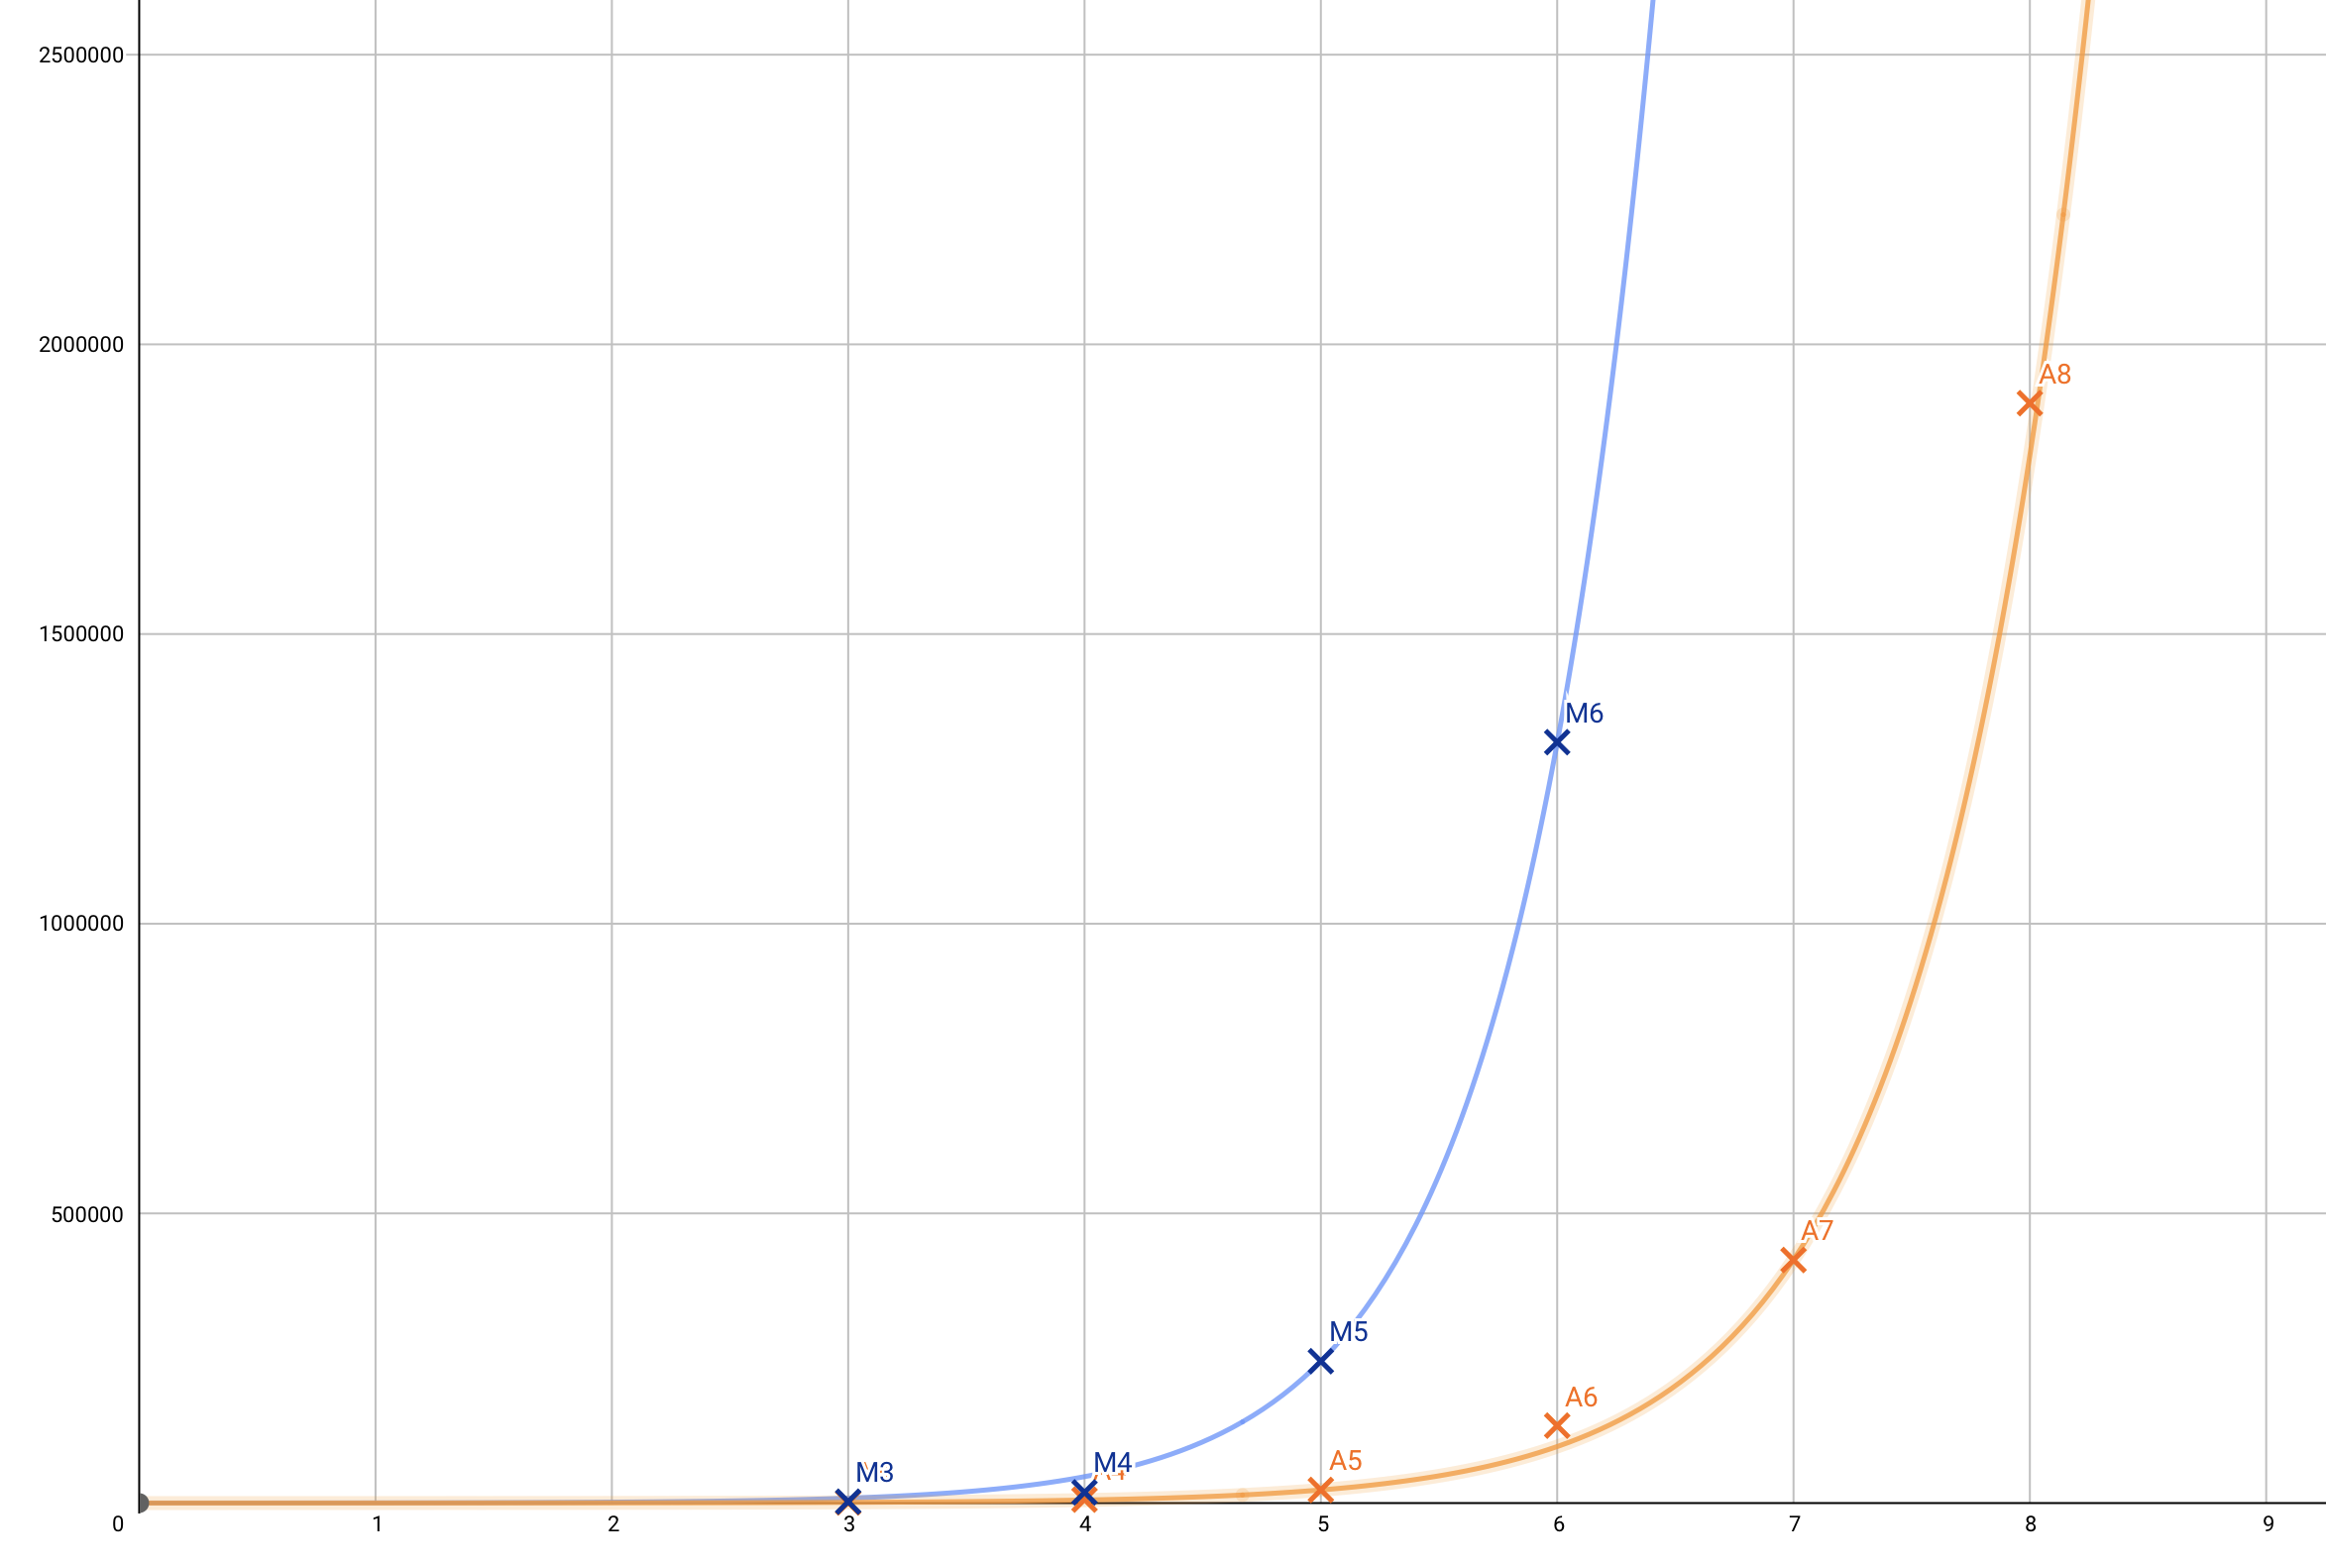
\includegraphics[width=0.7\linewidth]{pics/statistic-graph}
    \captionof{figure}[Suchbaumtiefen in Koordinaten]{Suchbaumtiefen in ein Koordinatensystem eingetragen}
    \label{fig:statistic-graph}
\end{minipage}

Der Aufwand, alle m\"oglichen Spielzust\"ande zu vergleichen, w\"achst bei beiden Verfahren exponentiell mit der Anzahl der Suchbaumtiefe.
Jedoch bewirkt das Alpha-Beta-Pruning eine gestauchtere Kurve als der Minimax-Algorithmus ohne Alpha-Beta-Pruning.

Bei gleicher Anzahl an bewerteten Feldern wird mit Alpha-Beta-Pruning der Suchbaum tiefer analysiert und dadurch mehr Z\"uge miteinander verglichen.
Das f\"uhrt dazu, dass bei gleichem Zeitaufwand (\corresponds gleiche Anzahl an analysierten Spielzust\"anden) das beste Ergebnis einer \underline{tieferen} Suchbaumebene gefunden wird.

\newpage

Um diese Aussage adequate zu best\"atigen sind vier weitere Karten (siehe Abbildung~\ref{fig:additional-statistic-maps}) aufgef\"uhrt, bei denen erneut Tests durchgef\"uhrt werden.
Die Statistiken zum Vergleich der Algorithmen befindet sich jeweils unterhalb der textuellen Vorstellung der einzelnen Karten.
Die blaue Linie stellt hierbei immer den Minimax-Algorithmus und die orange Linie das Alpha-Beta-Pruning dar.

\textbf{Reversi Cuboid:}
Diese Map basiert auf dem Grundspiel von Reversi, jedoch sind hier vier Bereiche angeordnet.
Durch diese Anordnung ist diese Map fair und es gibt einige Spezialfelder, die jedoch erst im sp\"ateren Verlauf des Spieles erreichbar sind.
Durch diese Karte soll getestet werden wie sich 8-Spieler-Karten auf die beiden Algorithmen auswirkt.
Diese Karte wird aufgrund vieler Spieler auf Tiefe 4 durchlaufen.
Dabei wird als erster und zweiter Spieler der Client zum Testen der Algorithmen verwendet.
Die anderen Spieler verwenden den triviale Client, welcher zu Beginn des Semesters jedem Team ausgeh\"andigt wird.

\begin{minipage}{\linewidth}
    \centering
    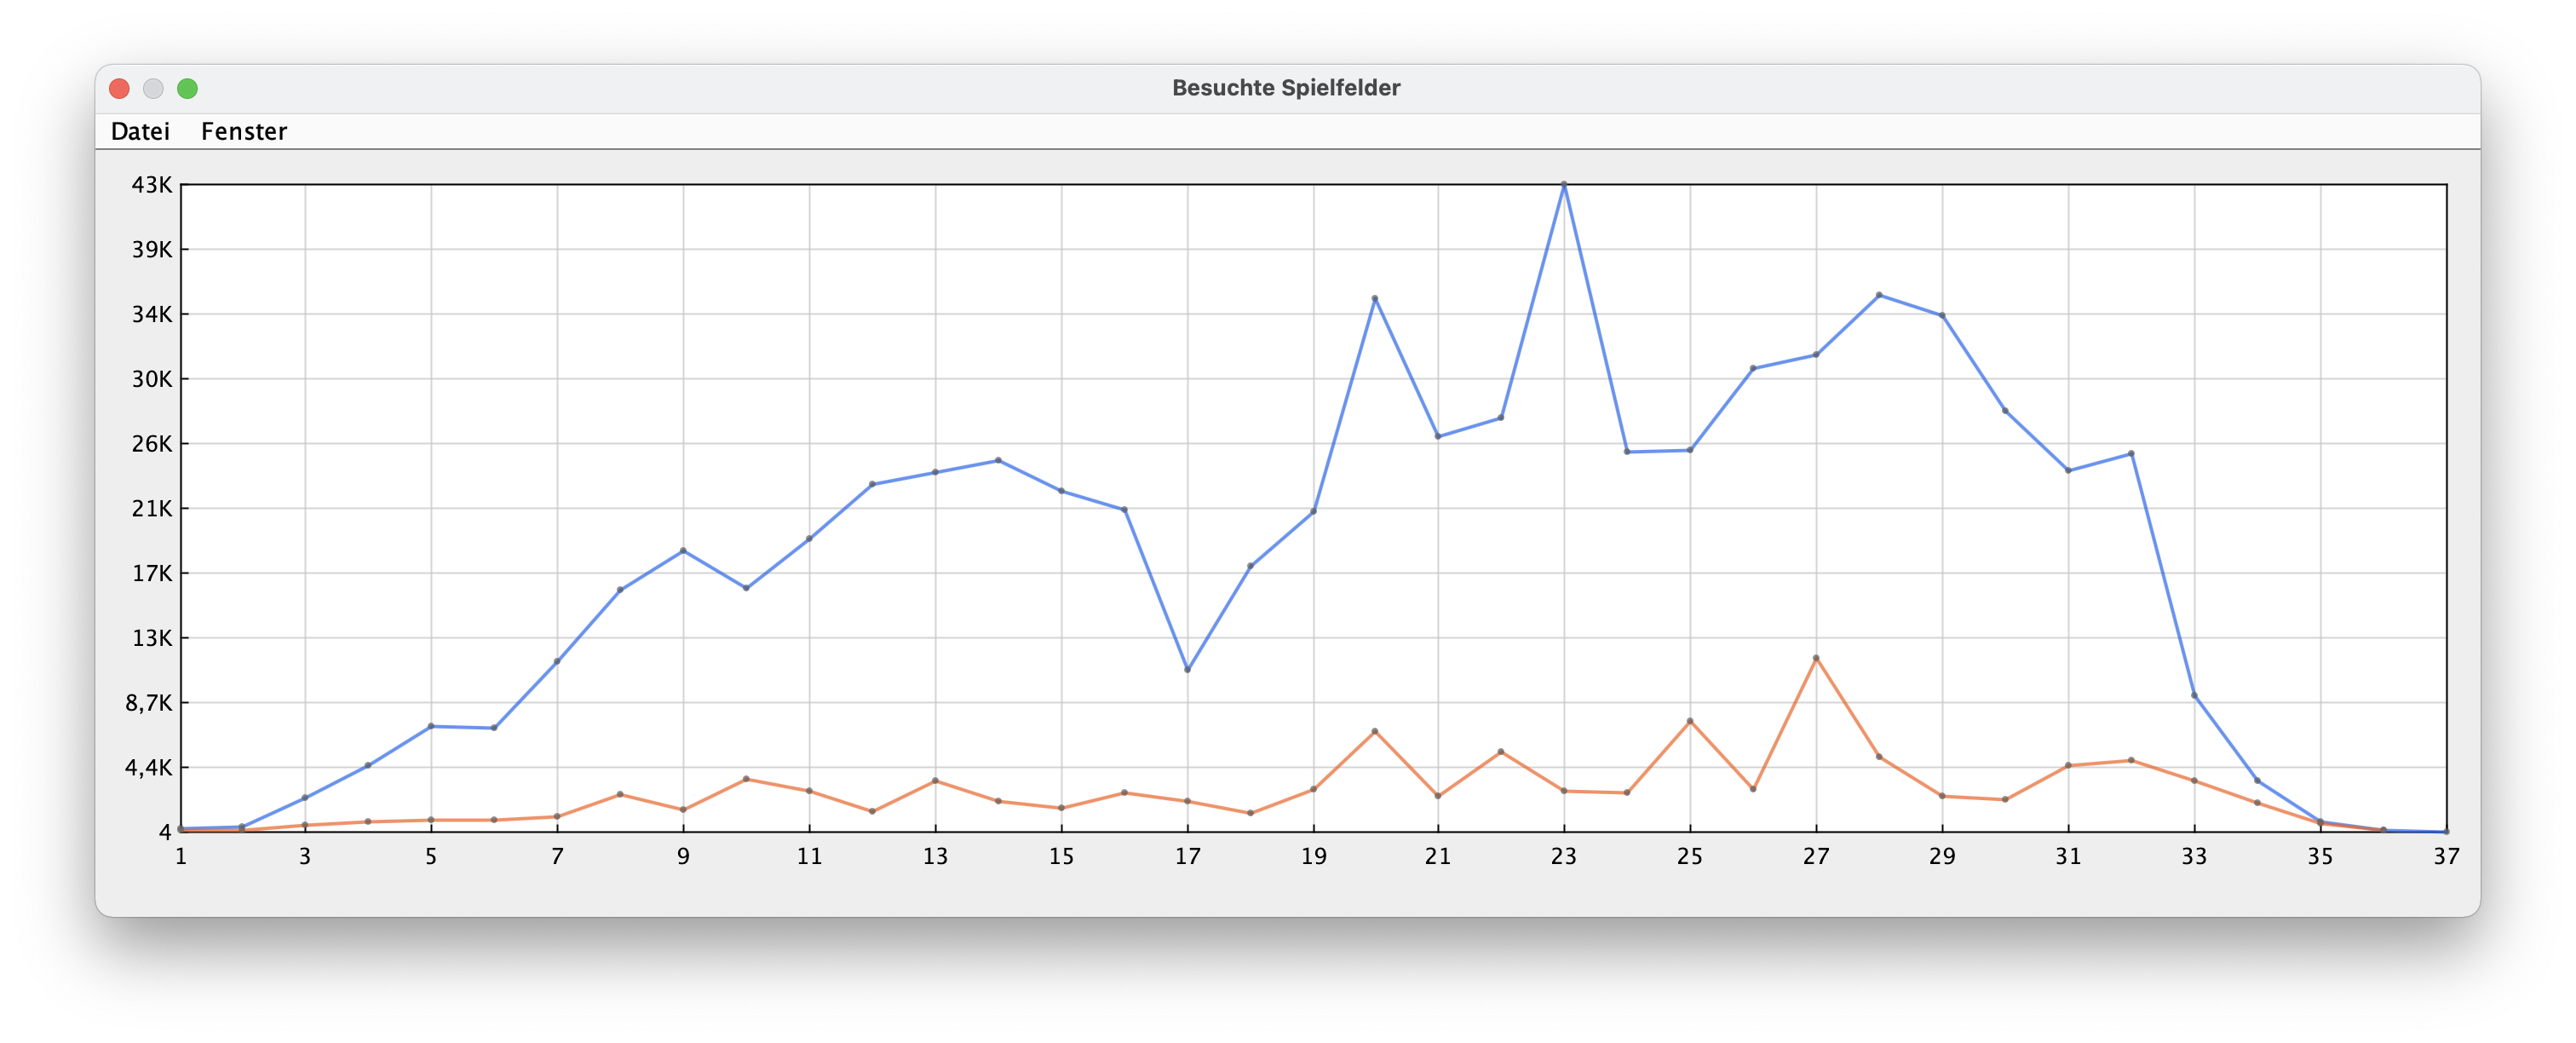
\includegraphics[width=0.9\linewidth]{statistic/CUBOID-01/ST-01-D4-LD}
    \captionof{figure}{Vergleich der Algorithmen auf der Karte Reversi Cuboid}
    \label{fig:statistic-graph-cuboid}
\end{minipage}
\vspace{1em}

\textbf{Cupcake:}
Diese Map hat bereits zu Beginn sehr viele unterschiedliche Startpositionen.
Was dazu f\"uhrt, dass der Suchbaum bereits zu Beginn sehr breit ist und somit sehr stark anw\"achst.
Er beeinhaltet jedoch keine Transitionen oder Sonstige Spezialfelder, wodurch die Anzahl damit jedoch zu einem gewissen Teil eingeschr\"ankt werden.
Die Karte wird auf Tiefe 4 durchlaufen.

\begin{minipage}{\linewidth}
    \centering
    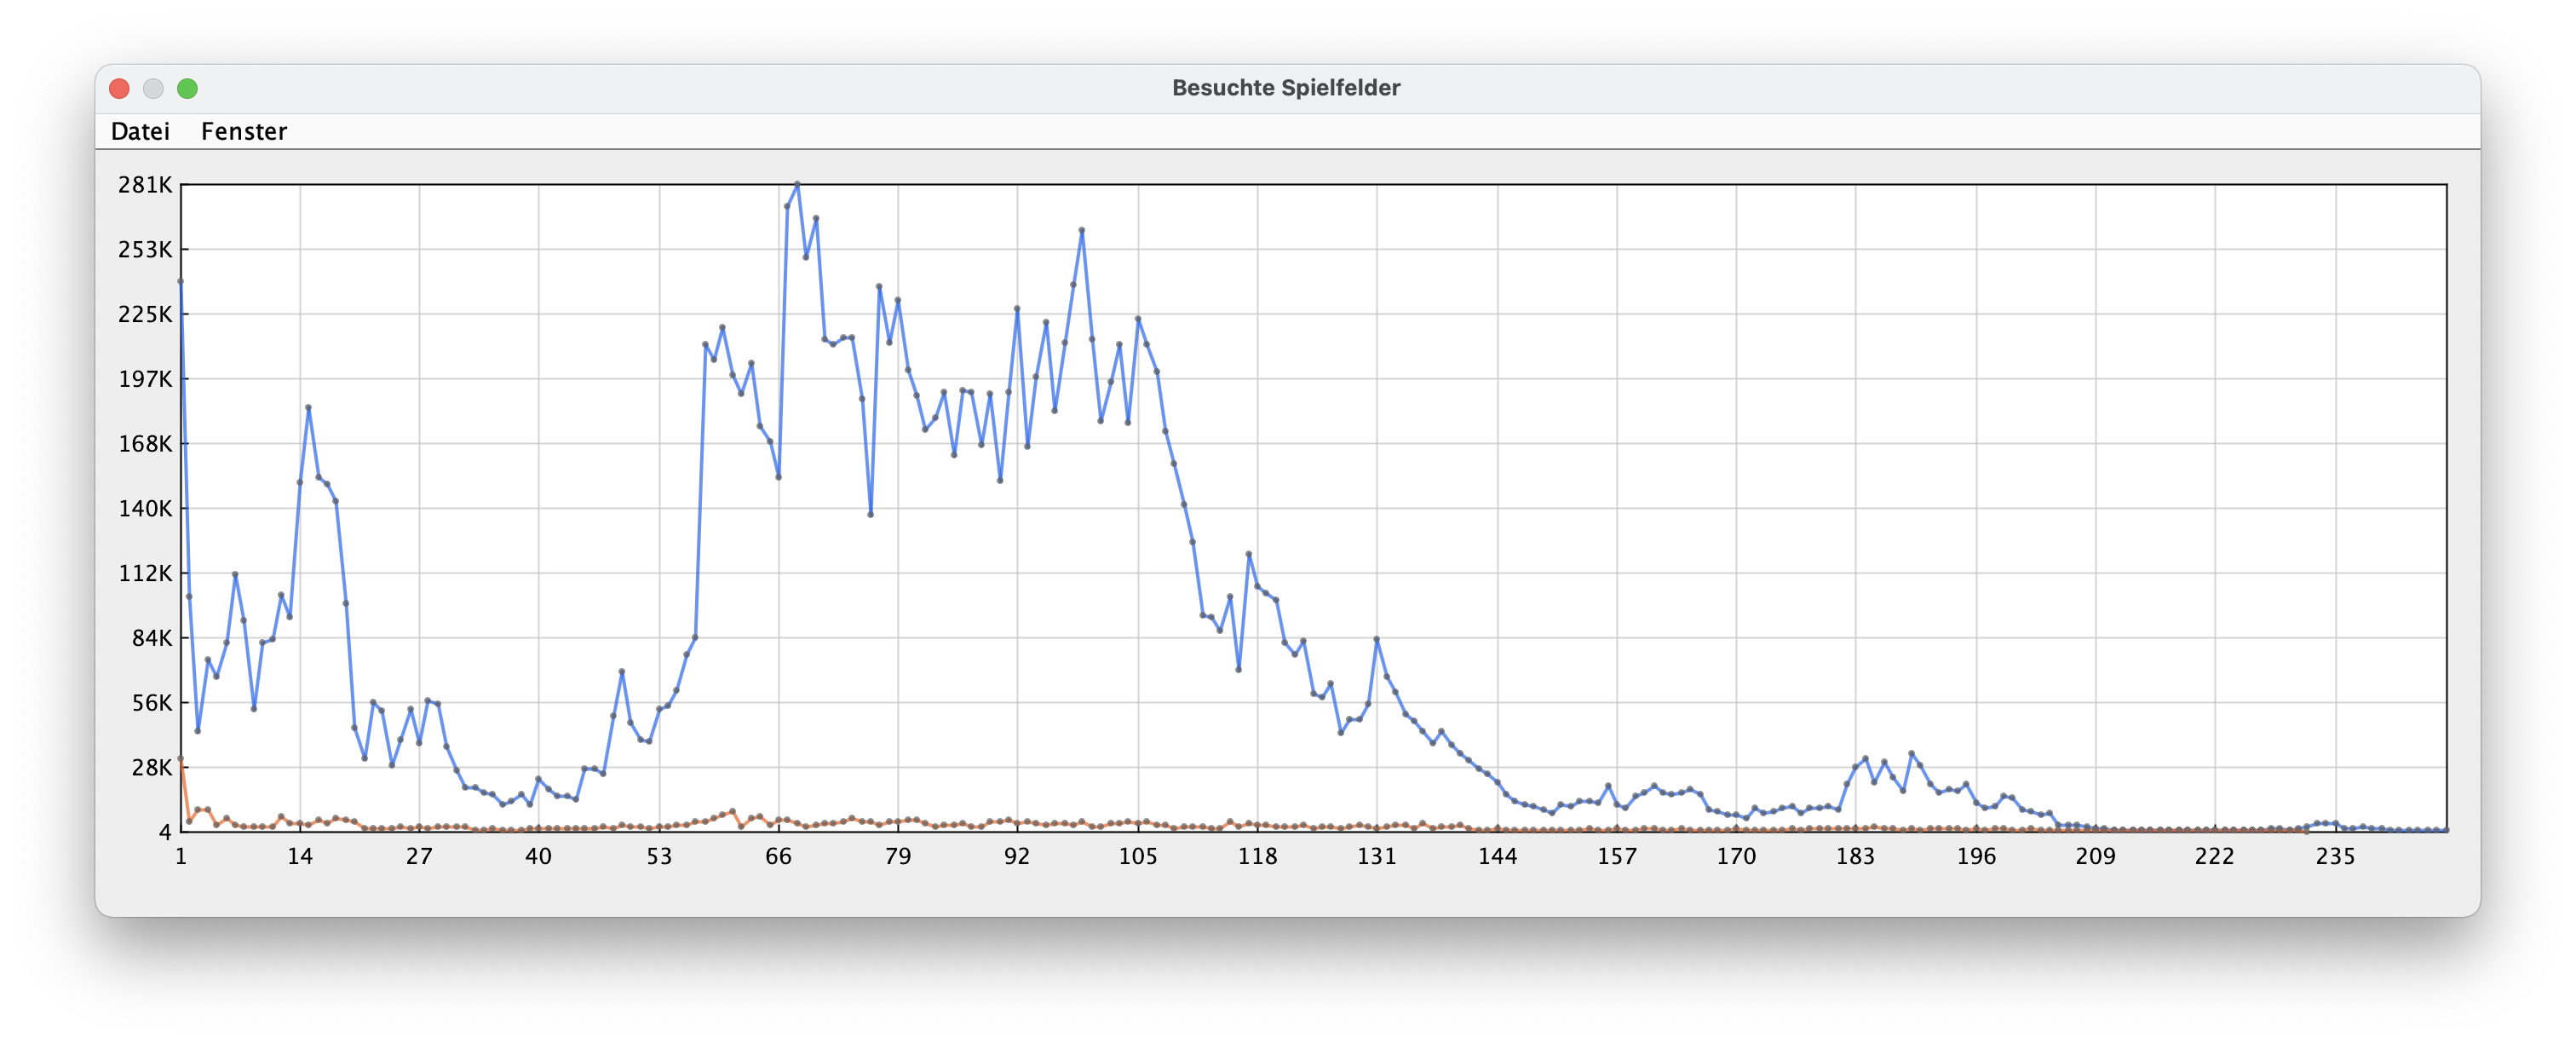
\includegraphics[width=0.9\linewidth]{statistic/CUP-01/ST-01-D4-LD}
    \captionof{figure}{Vergleich der Algorithmen auf der Karte Cupcake}
    \label{fig:statistic-graph-cupcake}
\end{minipage}
\vspace{1em}

\textbf{Dog Extended:}
Bei der Dog Extended Karte handelt es sich um die Karte, die f\"ur alle Abgaben w\"ahrend dem Semester verwendet wird.
Aus diesem Grund wird auch die Map Dog Extended bei diesem Test \"uberpr\"uft.
In dieser Karte sind Transitionen sowie alle m\"oglichen Spezialsteine integriert um alle Abh\"anigkeiten zu testen.
Diese Karte wird auf Tiefe 5 durchlaufen.

\begin{minipage}{\linewidth}
    \centering
    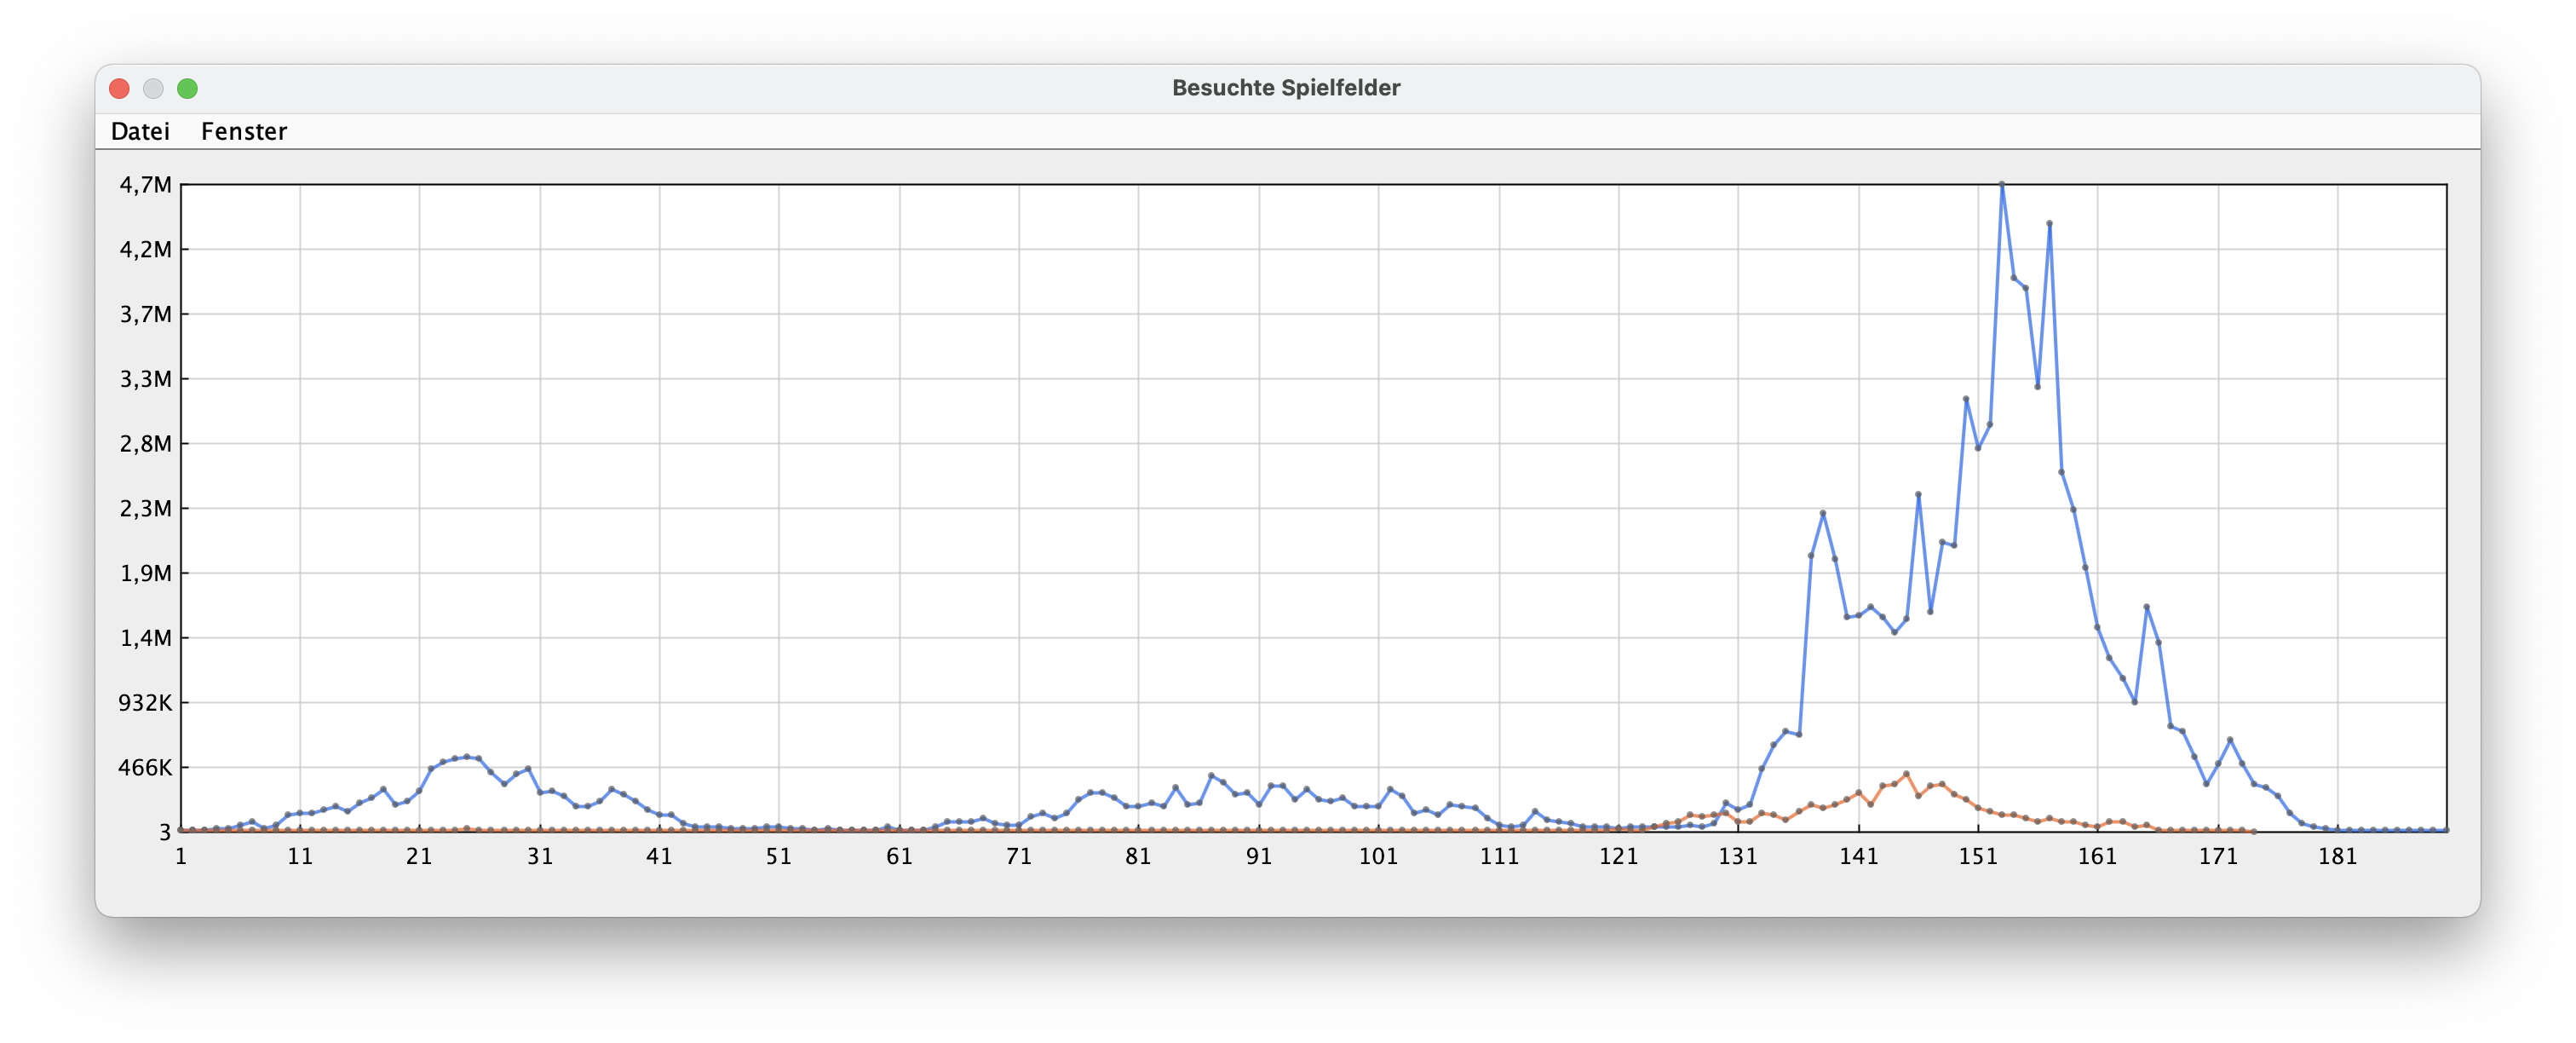
\includegraphics[width=0.9\linewidth]{statistic/DOG-02/ST-01-D4-LD}
    \captionof{figure}{Vergleich der Algorithmen auf der Karte Dog Extended}
    \label{fig:statistic-graph-dog}
\end{minipage}
\vspace{1em}

\textbf{Europa:}
Die Europa Karte ist eine sehr gro\"se Map bei der jedoch viele Stellen aus L\"ochern bestehen und es zudem eine Menge an Kanten und Ecken gibt.
Dadurch wird die Spielfeldgewichtung unter Probe gestellt um zu testen ob es hierbei zu starken Abweichungen kommt, da die Gewichtung hier oft gleiche Ergebnise liefern k\"onnte und somit wenig weggek\"urzt werden kann.
Diese Karte wird auf Tiefe 3 durchlaufen, da es eine sehr gro"se Karte mit drei Spielern ist.
Dabei wird als erster Spieler der triviale Client verwendet.

\begin{minipage}{\linewidth}
    \centering
    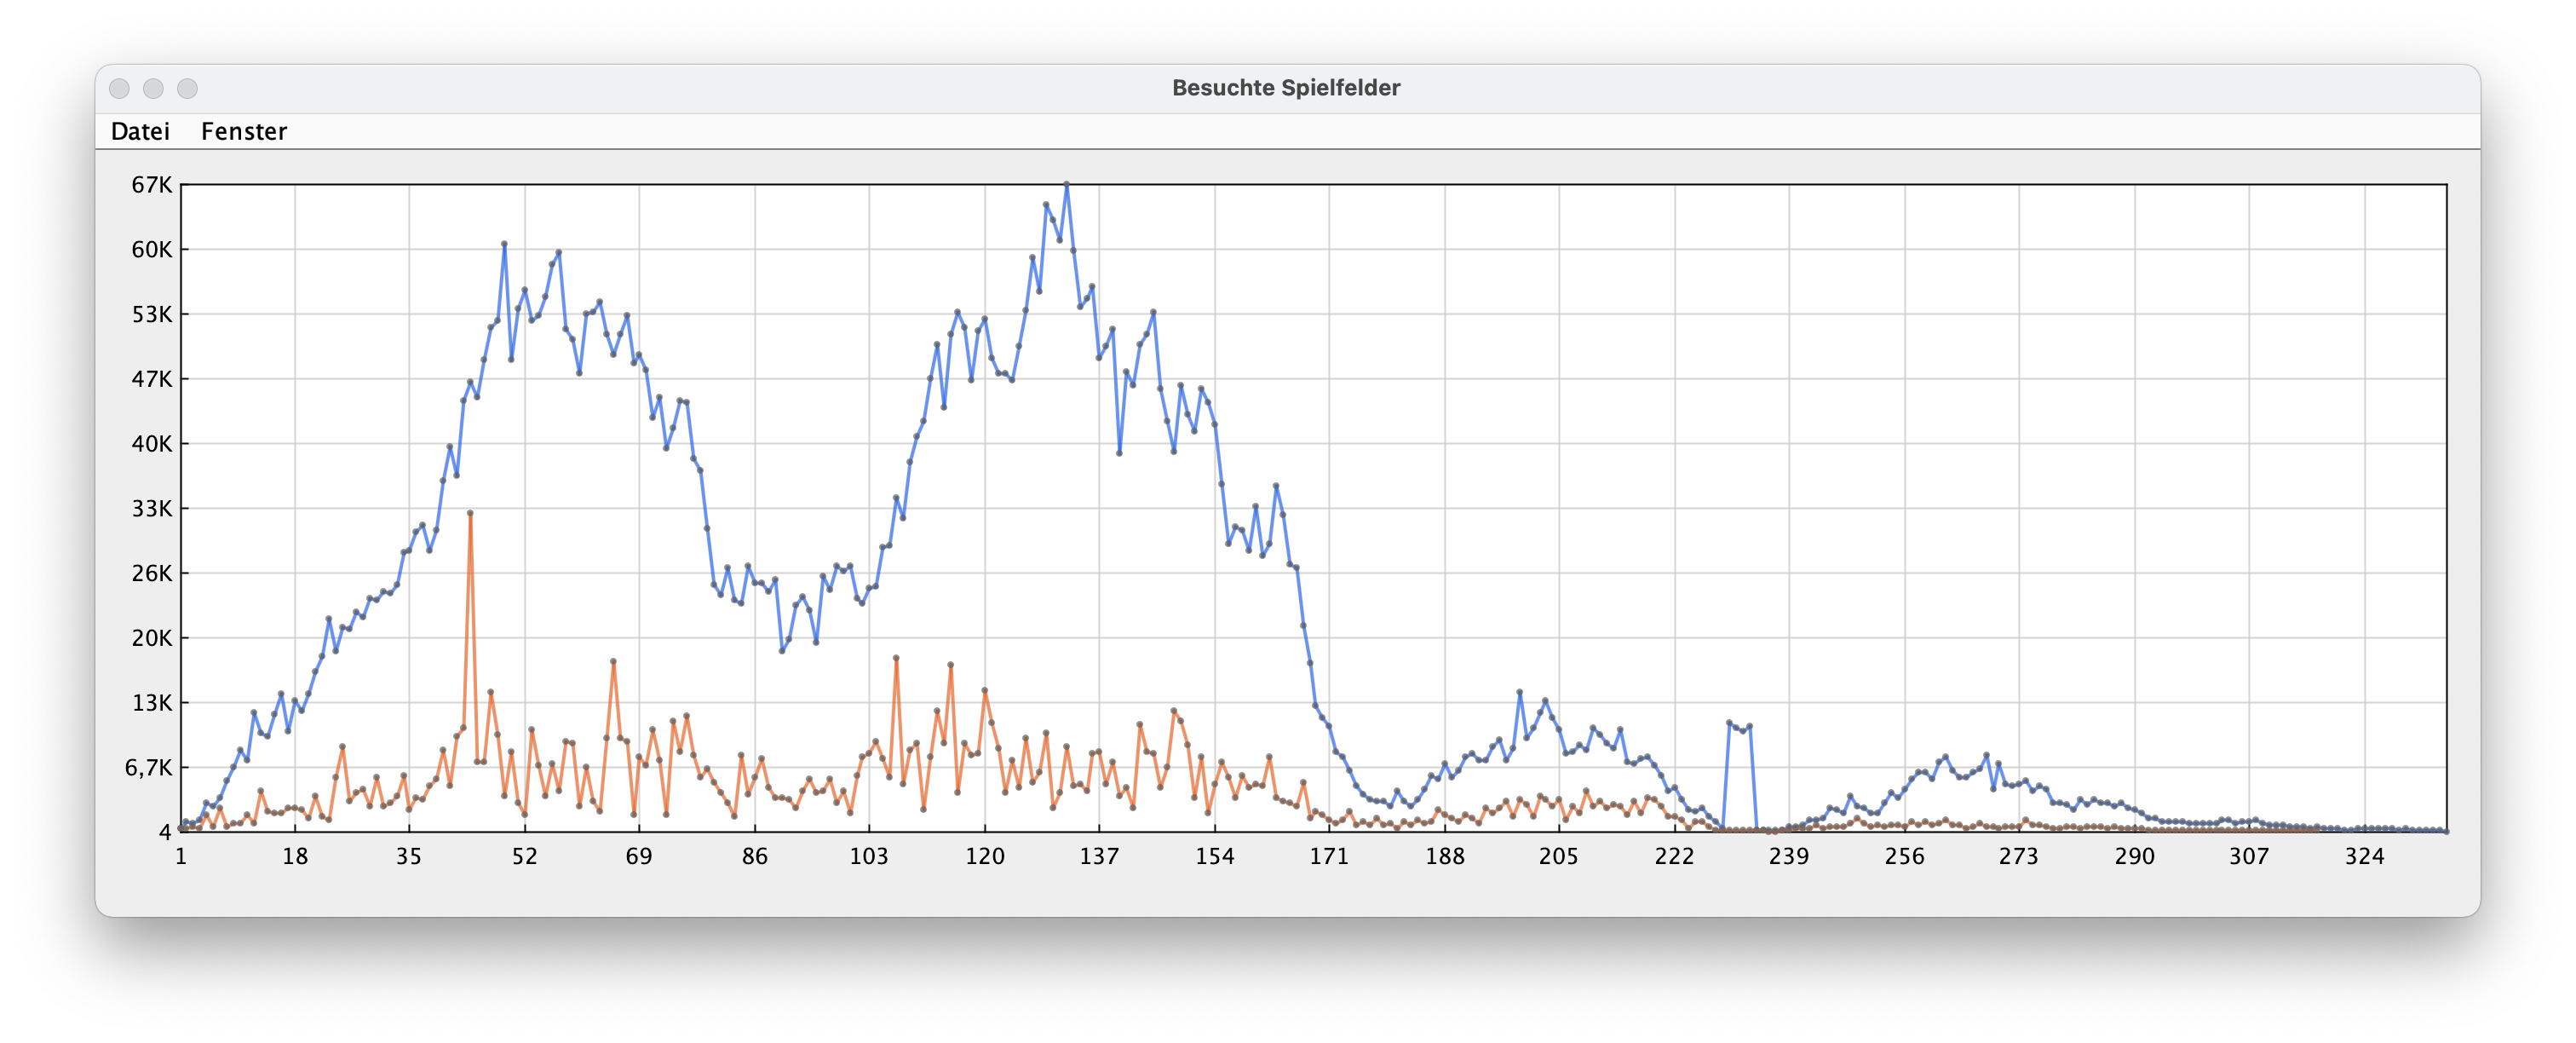
\includegraphics[width=0.9\linewidth]{statistic/EUROPA-02/ST-01-D3-LD}
    \captionof{figure}{Vergleich der Algorithmen auf der Karte Europa}
    \label{fig:statistic-graph-europa}
\end{minipage}
\vspace{1em}

\vspace{1em}
\begin{table}[!h]
    \centering
    \begin{tabular}{|l|c|c|c|}
        \hline
        \textbf{Karte} & \textbf{Tiefe} & \textbf{Alpha-Beta} & \textbf{Minimax}\\
        \hline
        Cupcake & 4 & 30.142 & 281.694\\
        \hline
        Reversi Cuboid & 6 & 11.459 & 48.656\\
        \hline
        Dog Extended & 5 & 978.310,5 & 4.357.785\\
        \hline
        Europa & 3 & 34.365 & 64.316,5\\
        \hline
    \end{tabular}
    \caption{Tabellarischer Vergleich der aufgef\"uhrten Statistiken (Ergebnisse wurden geglättet)}
    \label{tab:additional-search-depth}
\end{table}

Betrachtet man nun alle aufgef\"uhrten Karten kann man zwar jeweils einen Unterschied in der G\"ute des Alpha-Beta Prunings feststellen, jedoch wird hier klar ersichtlich, dass sich bei jeder getesteten Karte ein gewisser Leistungsvorteil ergibt.
Das Team hat sich genau aus diesen Gr\"unden dazu entschieden, auf jeder Karte standardm\"a"sig Alpha-Beta Purning zu aktivieren.

\vspace{1em}
\begin{figure}
    \centering
    \subfloat[Karte: Reversi Cuboid]{ 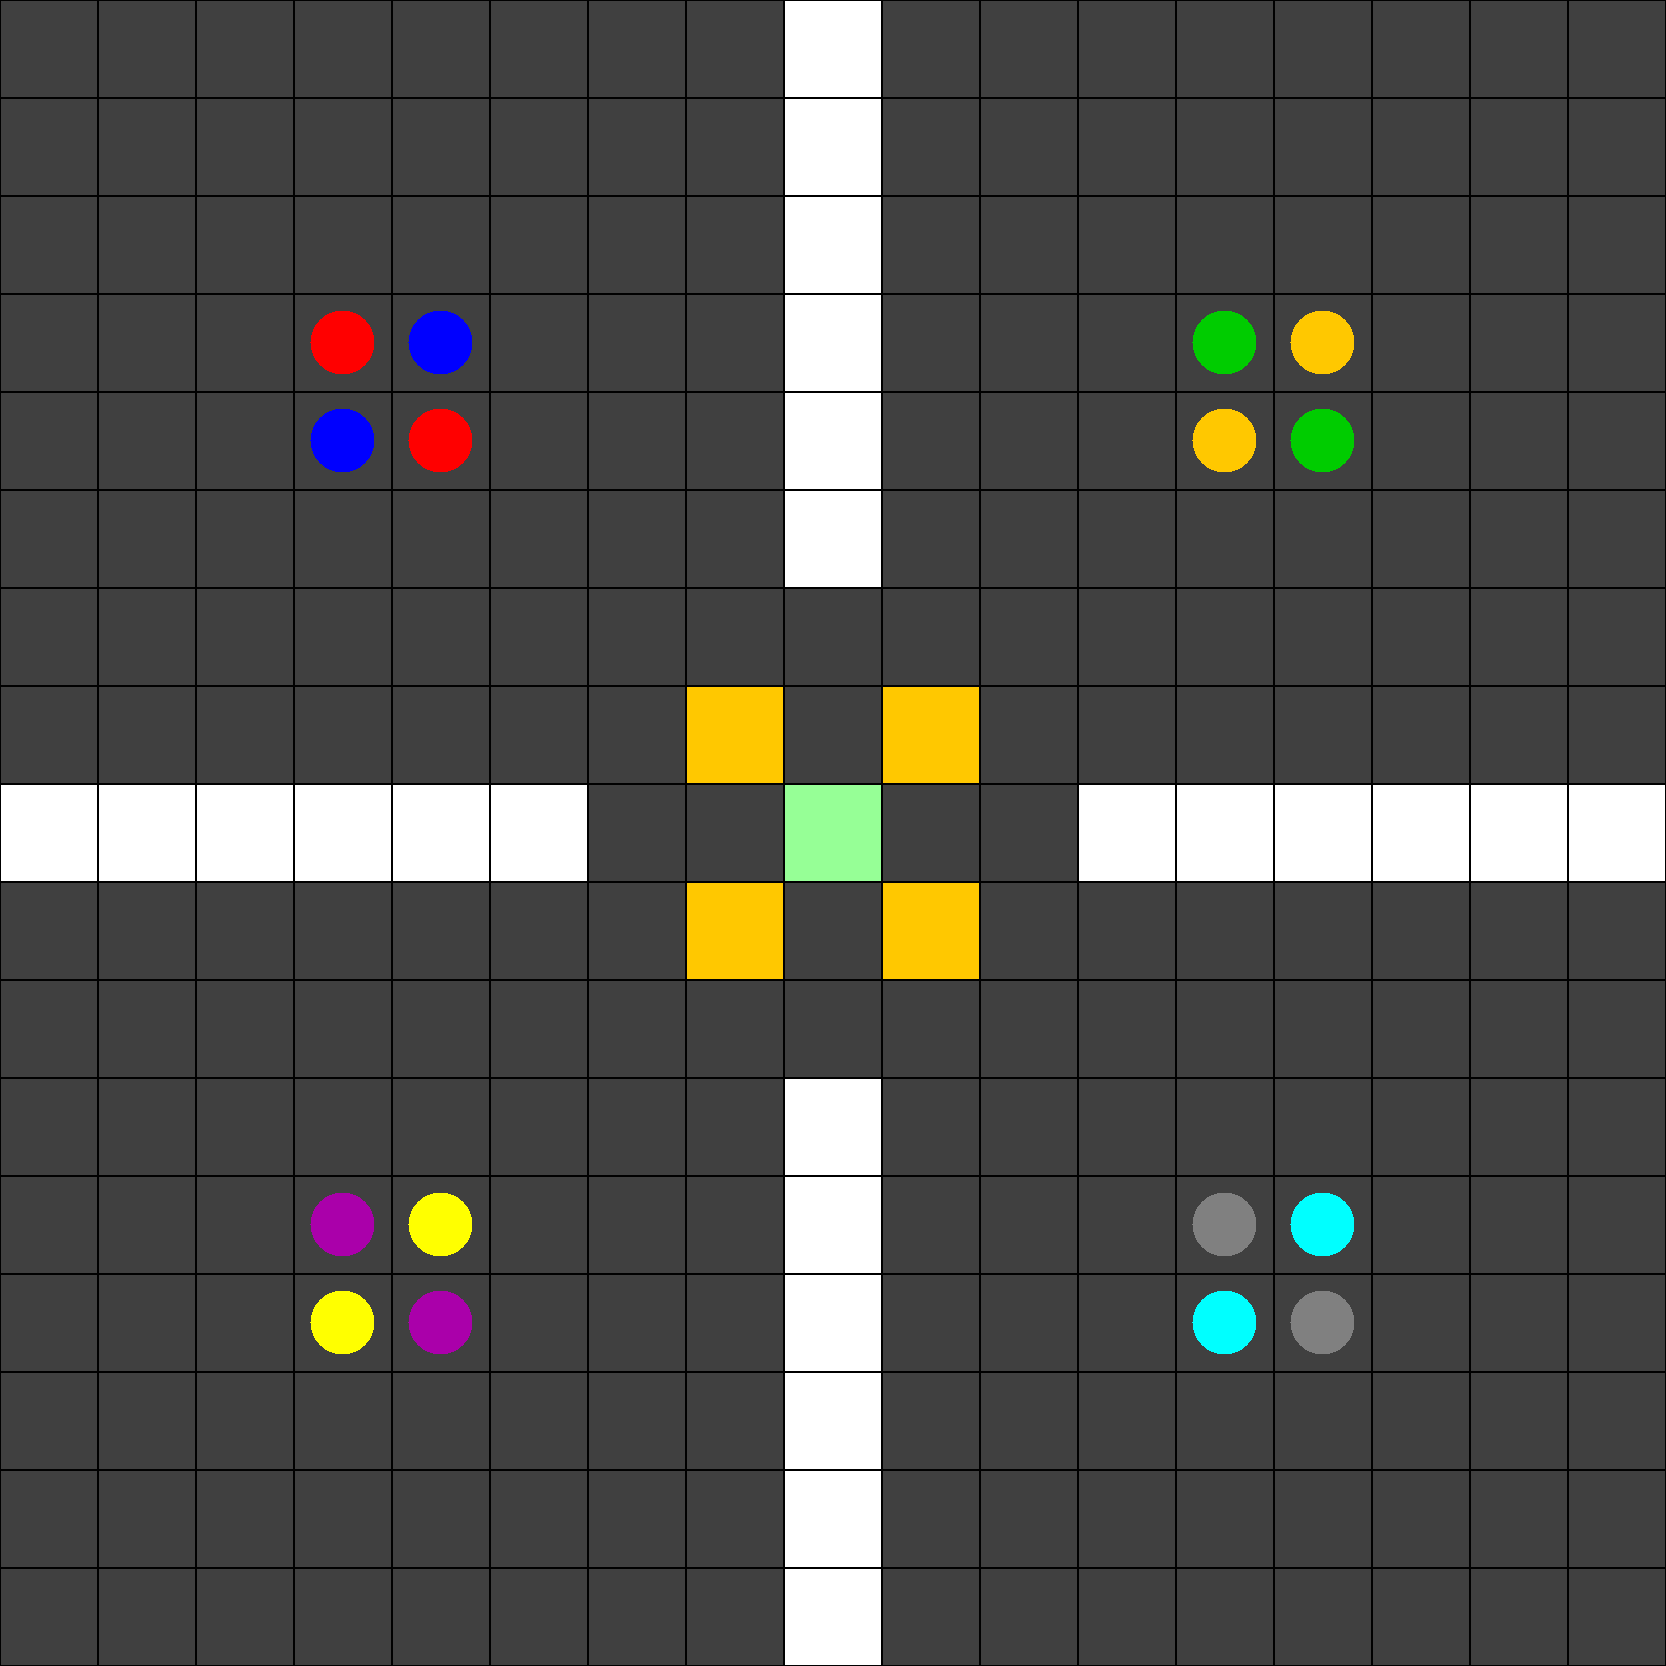
\includegraphics[width=0.5\linewidth]{pics/maps/reversi-cuboid} }
    \qquad
    \subfloat[Karte: Cupcake]{ 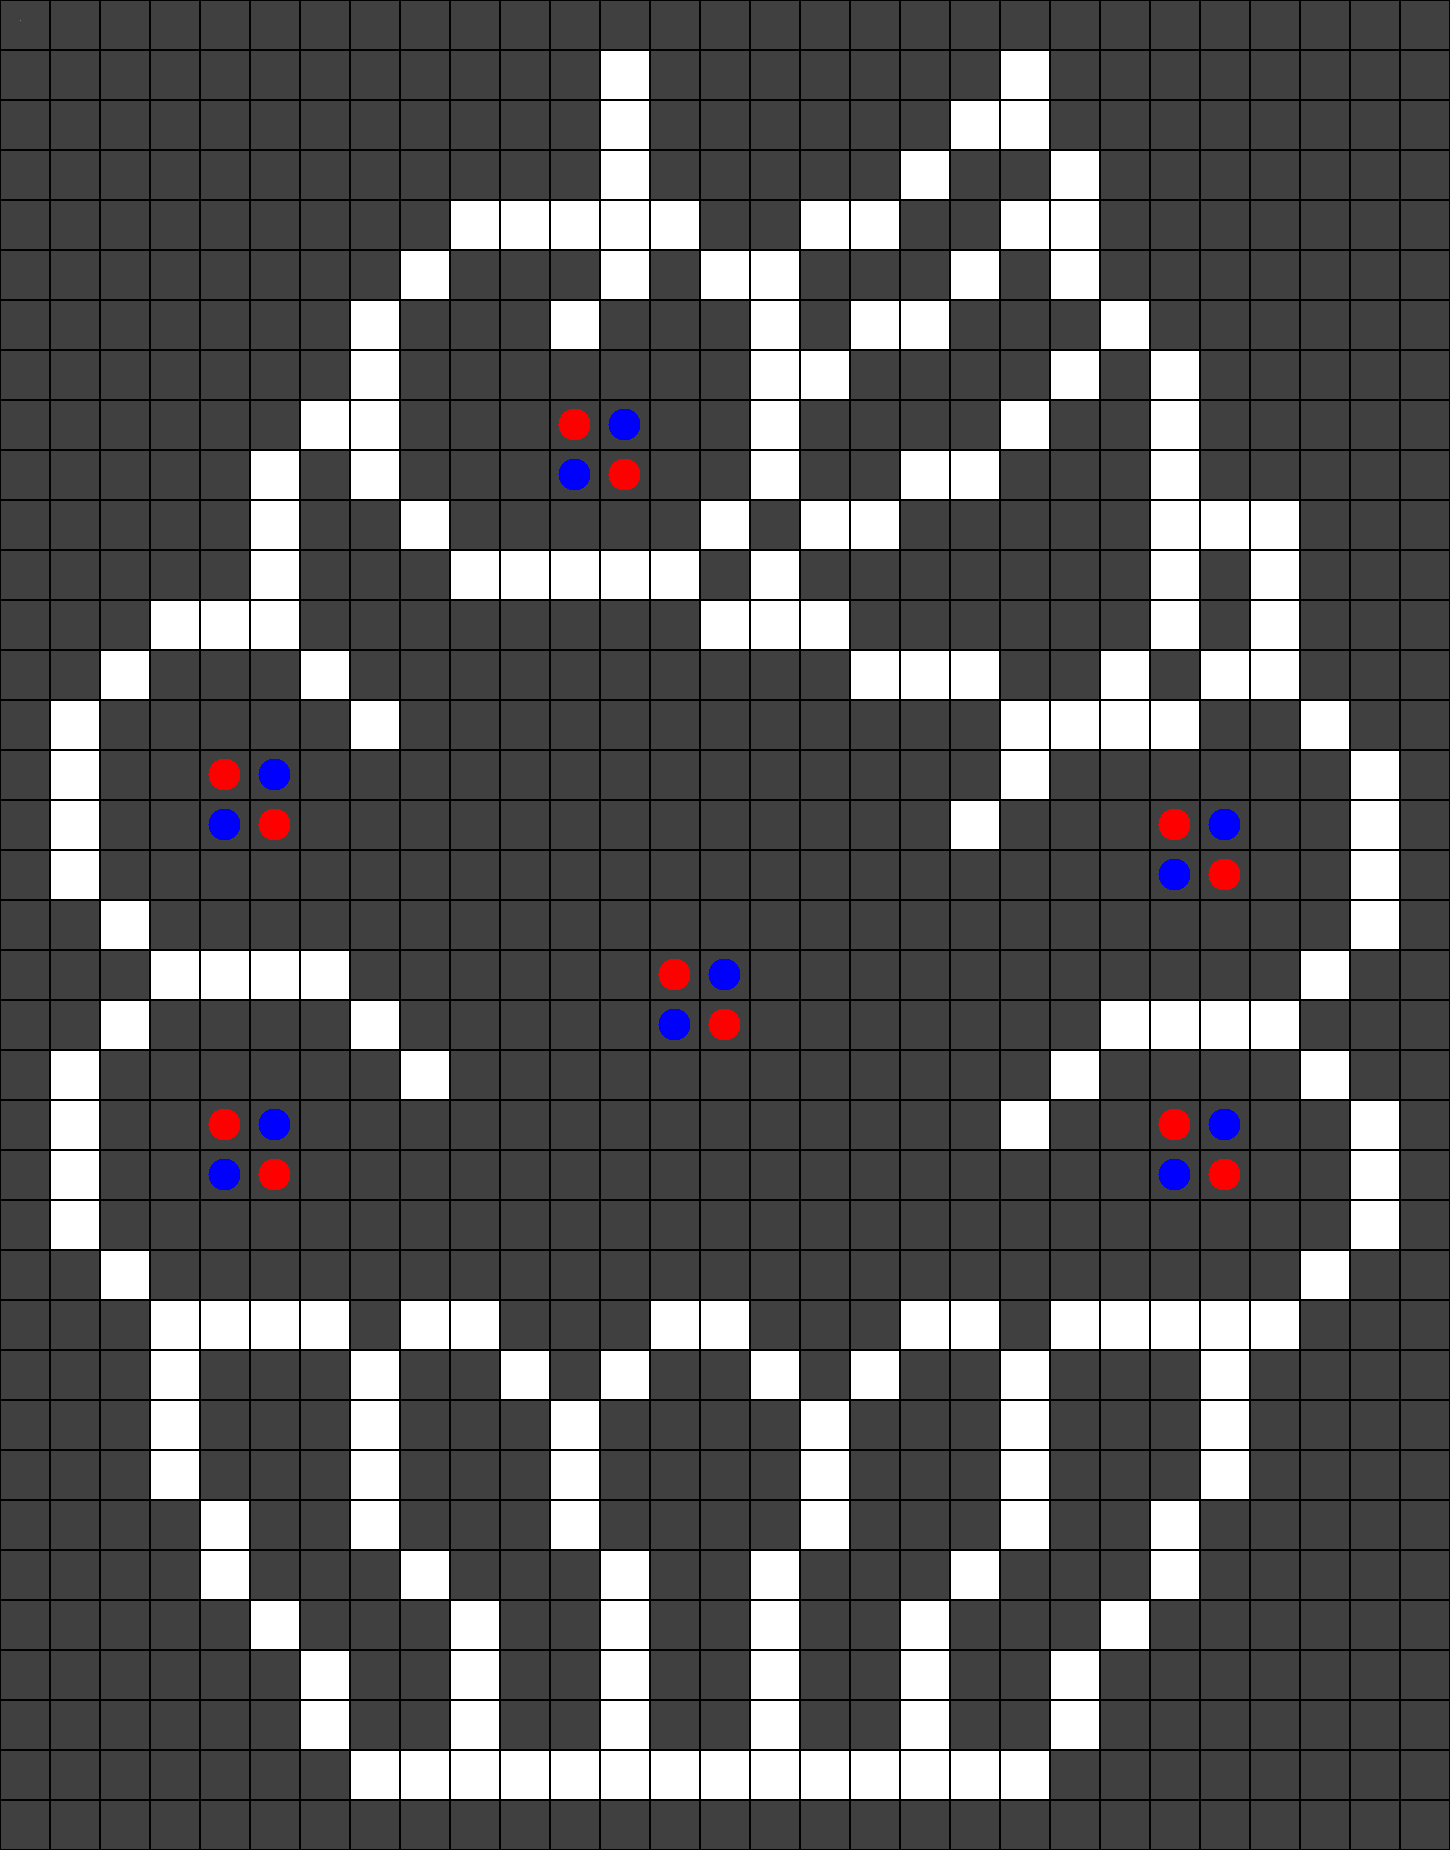
\includegraphics[width=0.4\linewidth]{pics/maps/cupcake} }
    \qquad
    \subfloat[Karte: Dog Extended]{ 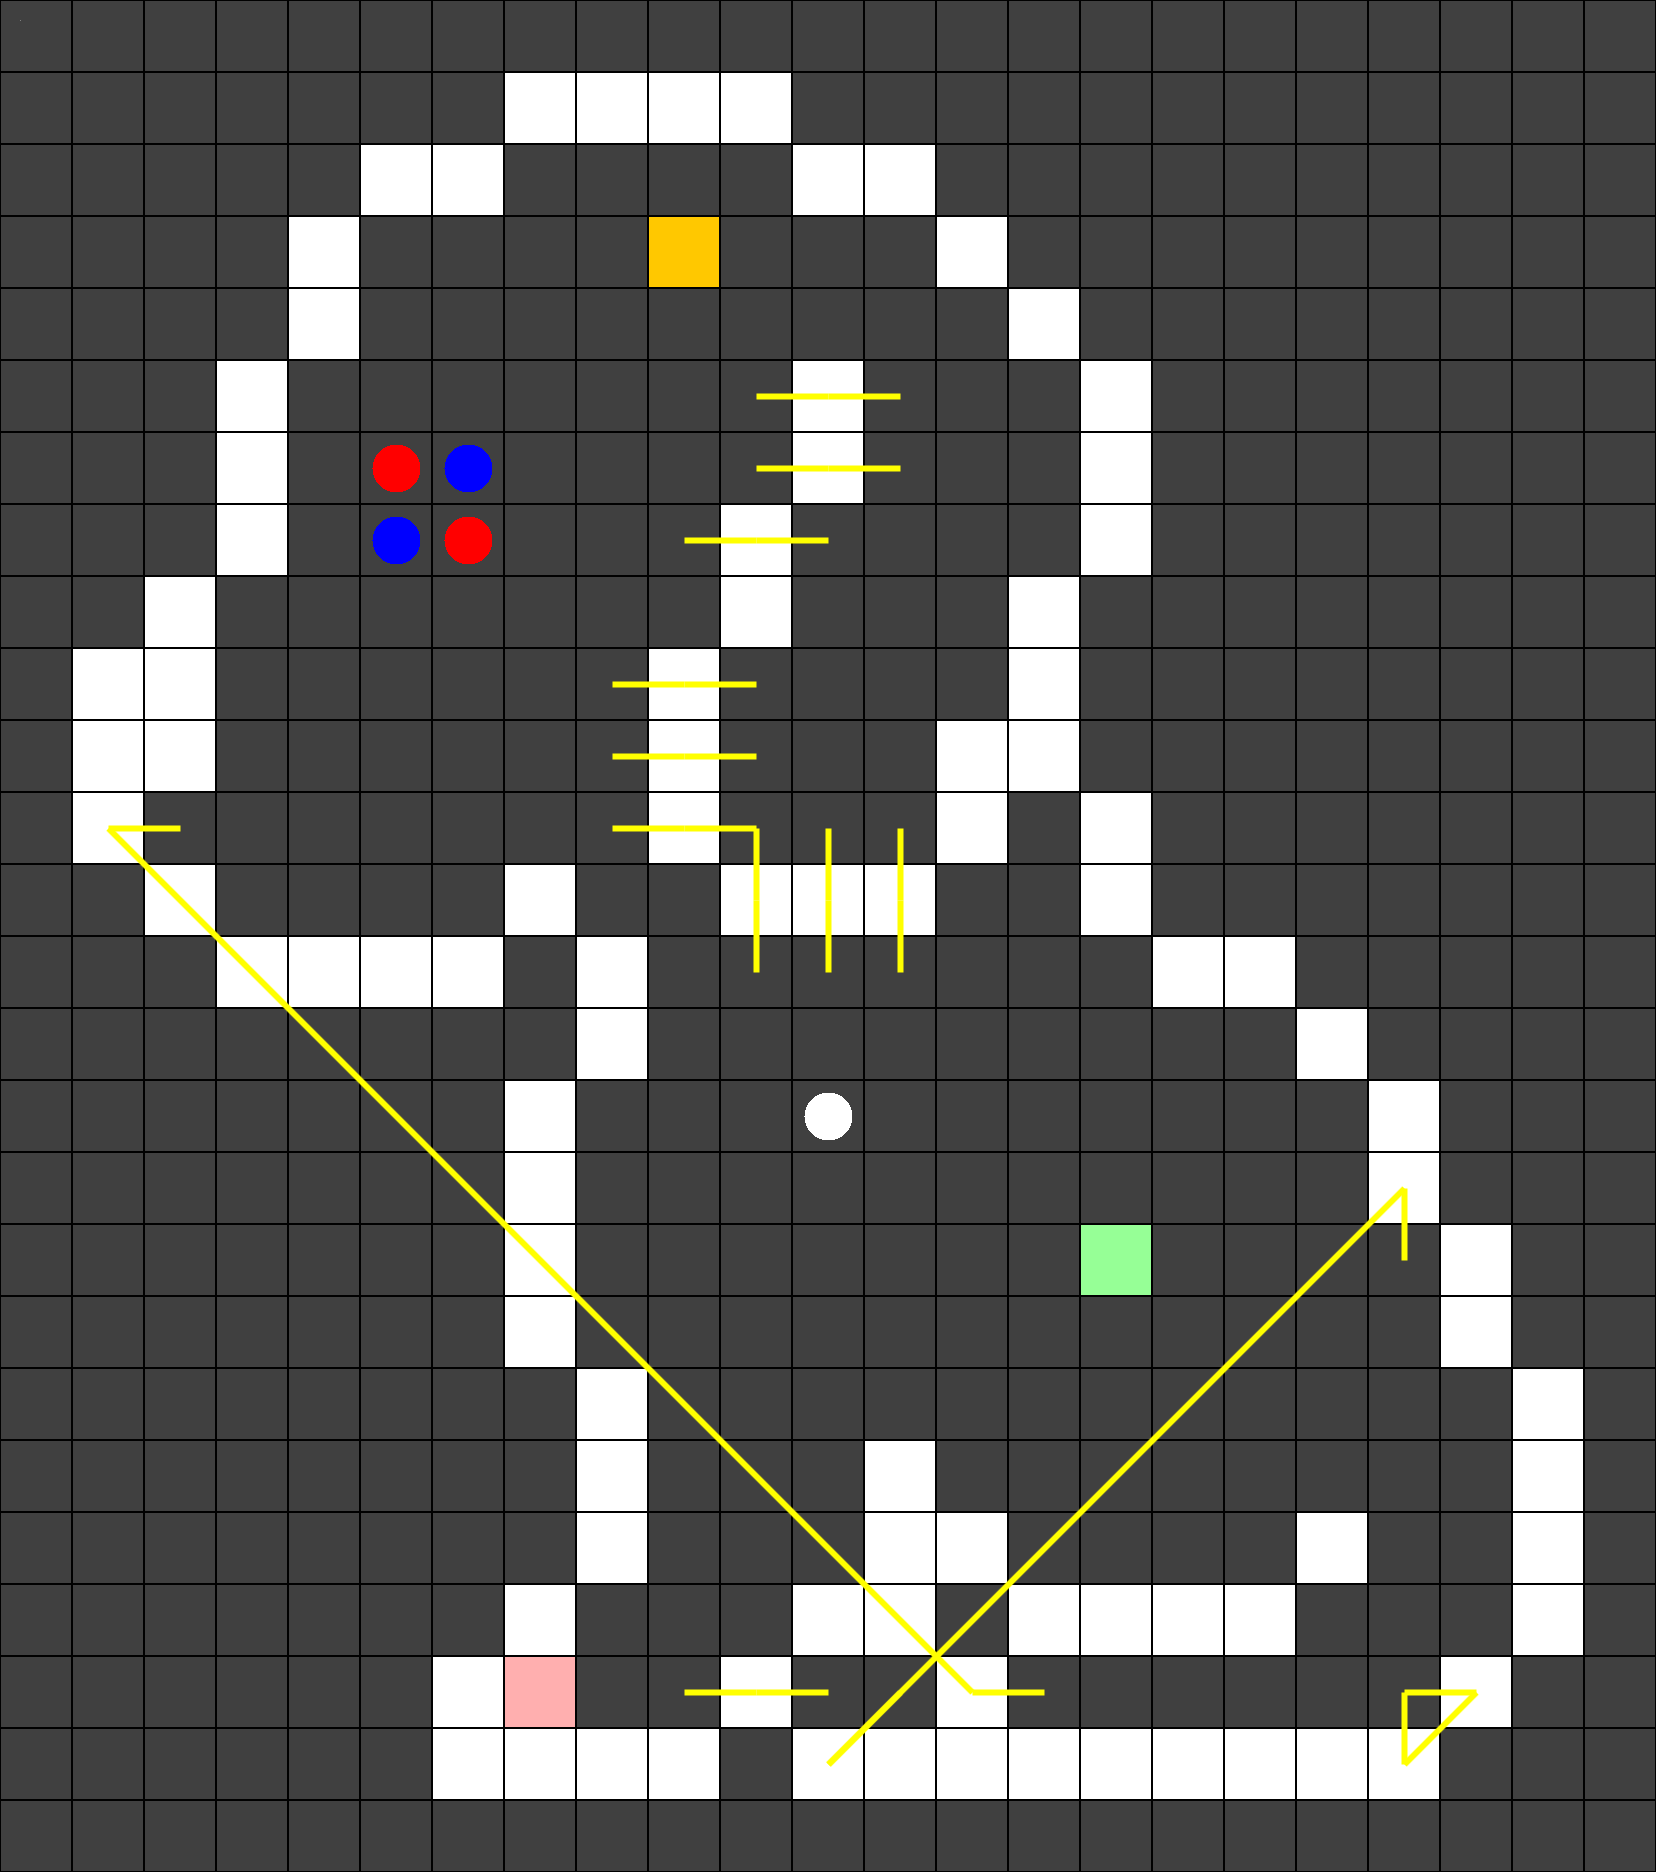
\includegraphics[width=0.4\linewidth]{pics/maps/dog-extended} }
    \qquad
    \subfloat[Karte: Europa]{ 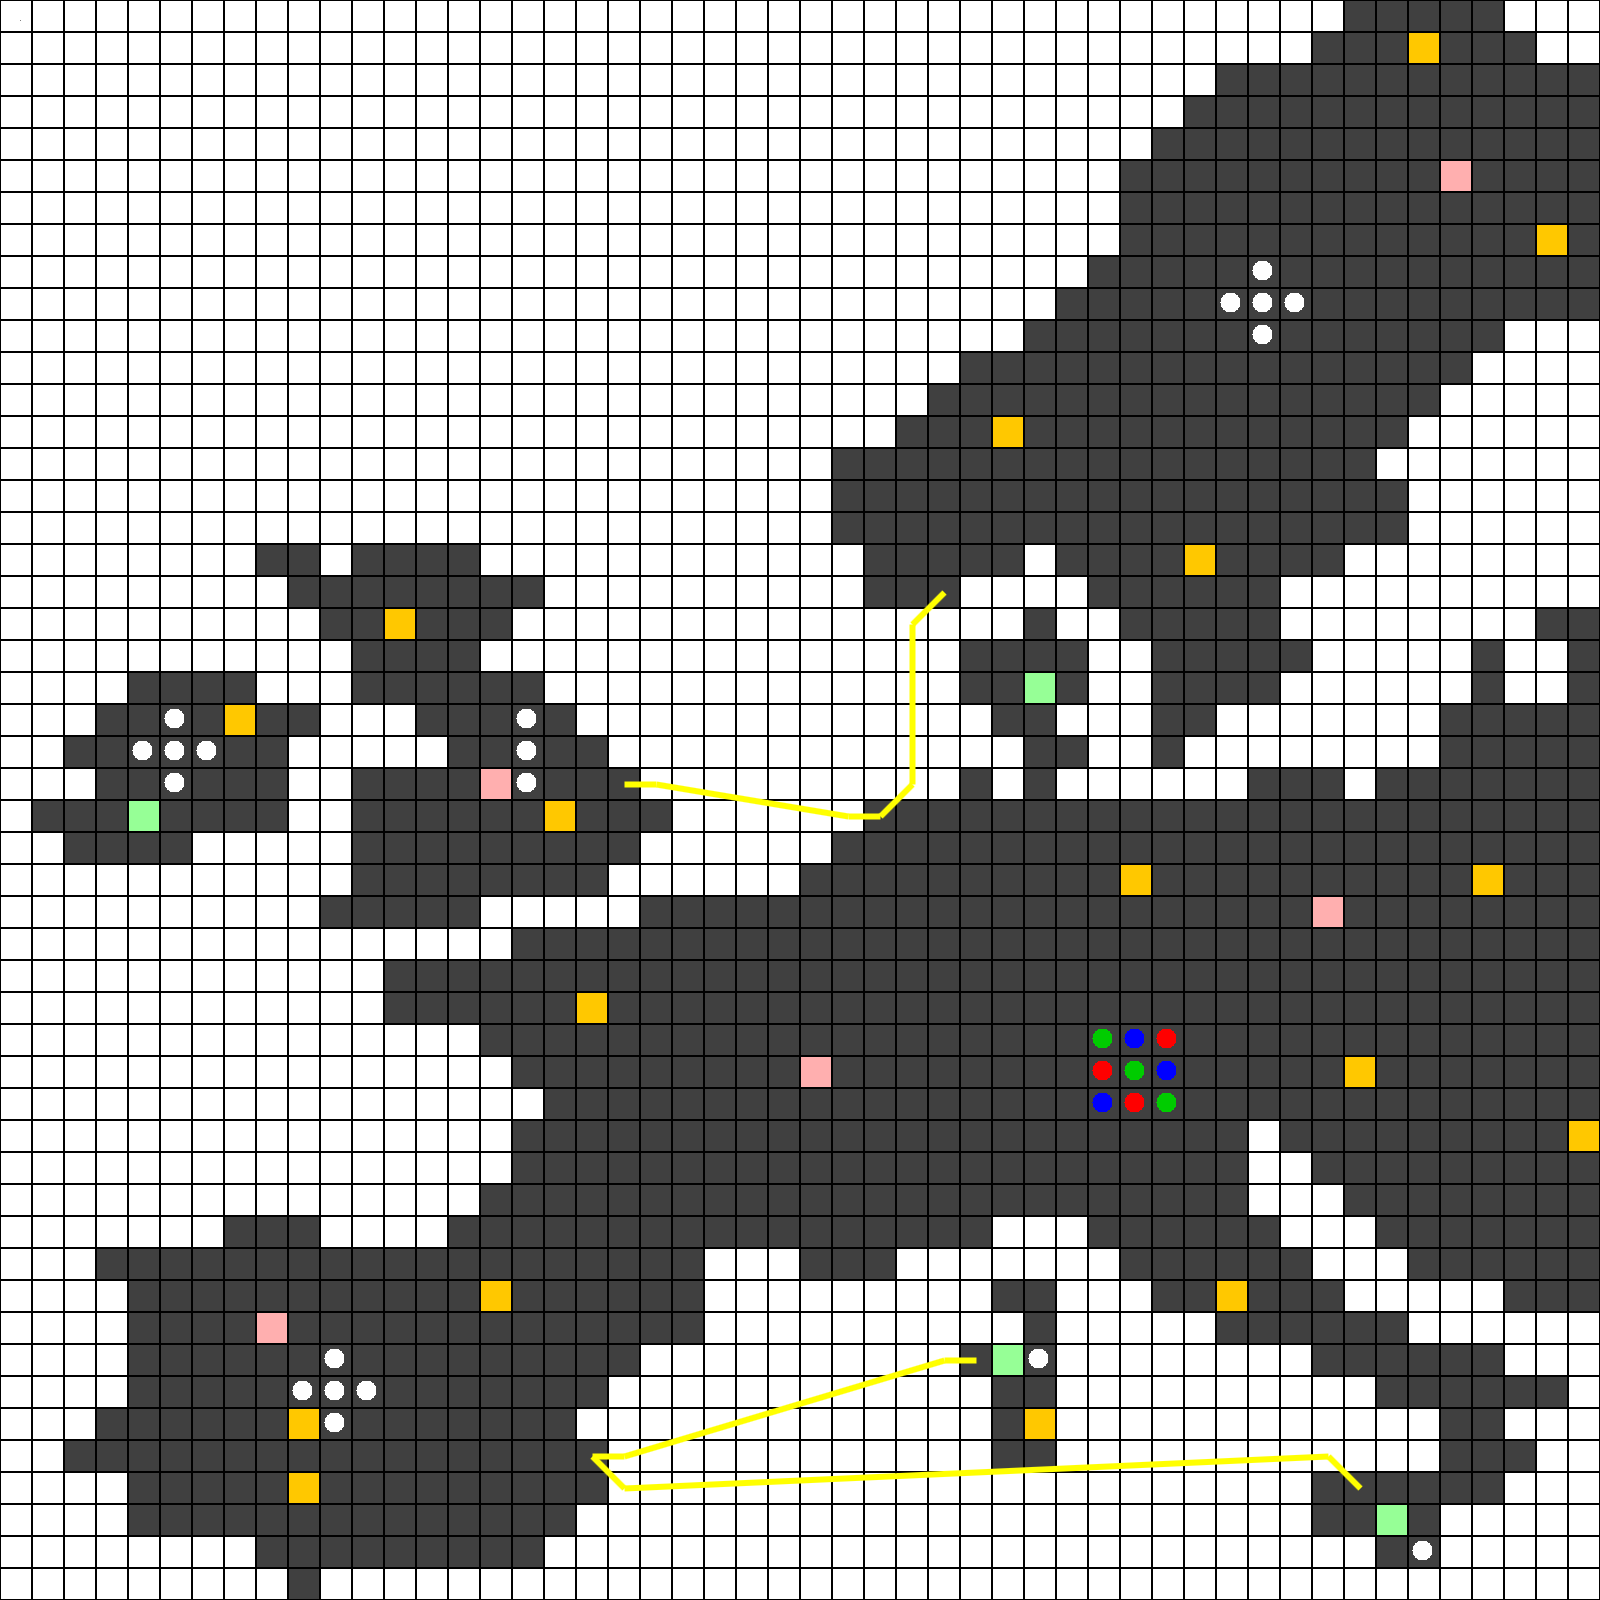
\includegraphics[width=0.5\linewidth]{pics/maps/europa} }

    \caption{Weitere Karten die f\"ur die Statistik verwendet werden}
    \label{fig:additional-statistic-maps}
\end{figure}


\bigskip
\newpage